\documentclass[12pt]{article}
%\usepackage{graphicx}
\usepackage[pdftex]{graphicx}
\usepackage{fancyhdr}
\usepackage[latin1]{inputenc}
\usepackage{moreverb}
\usepackage{amssymb}
%\usepackage[sectionbib]{natbib}
\usepackage[english]{babel}
\pagestyle{fancy}
\begin{document}


\fancyhead[LE,LO]{
\includegraphics[height=13pt]{molflow.png}}
\fancyhead[CE,CO]{}
%\fancyhead[RE,RO]{\bfseries\nouppercase\leftmark}
\fancyhead[RE,RO]{}
\fancyfoot[LO,LE]{}
\fancyfoot[RO,RE]{}
\fancyfoot[CO,CE]{\thepage}
\renewcommand{\footrulewidth}{0.4pt}
\renewcommand{\headrulewidth}{0.4pt}




\title{A level0 to level1b database for Odin-SMR\\
       \vspace*{85mm}}
\author{
        Bengt Rydberg, bengt.rydberg@molflow.com\\
        Joakim M\"{o}ller, joakim.moller@molflow.com\\
        %Dept. of Geo and Space Sciences\\%\vspace*{10mm}
        %Chalmers University of Technology\\
        Gothenburg, Sweden\\
        }
%\date{Gothenburg, Sweden}

\begin{titlepage}
            
\includegraphics[width=0.3\textwidth]{molflow.png}
  \begin{flushright}
    \noindent\rule{\textwidth}{2pt}
    \vspace{1cm}
    \begin{huge}
      Calibration study of data from the  autocorrelators of Odin-SMR\\
    \end{huge}
      \vspace{1cm}
   \today\\
    \noindent\rule{\textwidth}{2pt}
    \vspace{1cm}\\
    \begin{minipage}[t]{0.3\textwidth}
    \end{minipage}%
    \begin{minipage}[t]{0.30\textwidth}
        Joakim M\"{o}ller\\
        Bengt Rydberg
    \end{minipage}%
    \begin{minipage}[t]{0.4\textwidth}
      \begin{flushright}
        joakim.moller@molflow.com
        bengt.rydberg@molflow.com
      \end{flushright}
\end{minipage}
  \vspace{8cm}
\end{flushright}
\end{titlepage}

\makeatletter\@addtoreset{section}{part}\makeatother%
%\renewcommand{\thepart}{\hbox to 4em{part \Roman{part}}}
\renewcommand{\thepart}{Part \Roman{part}}
\tableofcontents
\thispagestyle{empty}
\newpage
\setcounter{page}{1}

\graphicspath{{./figures/}}
    
%\chapter{Intro}
%text...
%\chapter{Background}
\section{Overview}
This report contains a collection of four individual smaller reports. 
The topic of each report is related to the calibration process of 
auto-correlator data from Odin-SMR.  

\clearpage
\newpage
%\renewcommand{\thepart}{\Roman{part}}

%\begin{part}{Zerolags, high altitude spectra, and sky signals}
\part*{Part I \newline
Zerolags, high altitude spectra, and sky signals}
\addcontentsline{toc}{part}{Part I  \newline Zerolags, high altitude spectra, and sky signals }
\fancyhead[RO,RE]{\bfseries Part I: Zerolags, high altitude spectra, and sky signals  }
\setcounter{section}{0}
\section{Overview}
This report contains figures related to the calibration
process of autocorrelator data from Odin-SMR.\\
\newline
Topics examined are:\\
\newline
zerolags (proportional to the power of the eight bands of the correlators) 
and temperature\\
can we understand the variation
of zerolags from various temperature information?
The answer is yes and no.
Occasionally the levels of zerolags changes which we can not
understand from temperature variations.
Except from these occasions the zerolags are correlated to temperature.\\
\newline
Spectral feature in high altitude spectrum\\
We have calibrated data with a slightly modified calibration scheme,
but we still see spectral feature in high altitude spectra.
It is shown that lower altitude spectrum also contains this
spectral feature, and it should be possible to remove this
spectral feature as a frequency dependent tspill contribution\\
\newline
Calibration of sky signals\\
as a healty check of the calibration routine we have calibrated
sky signals. On average calibrated sky signals are very close to 0 k,
but can deviate significantly. Calibrated sky signals around
a target signal can potentially be used as a quality flag.
 
    



\clearpage
\newpage

\section{Zerolags and temperatures}
\begin{figure}[!t]
\centering
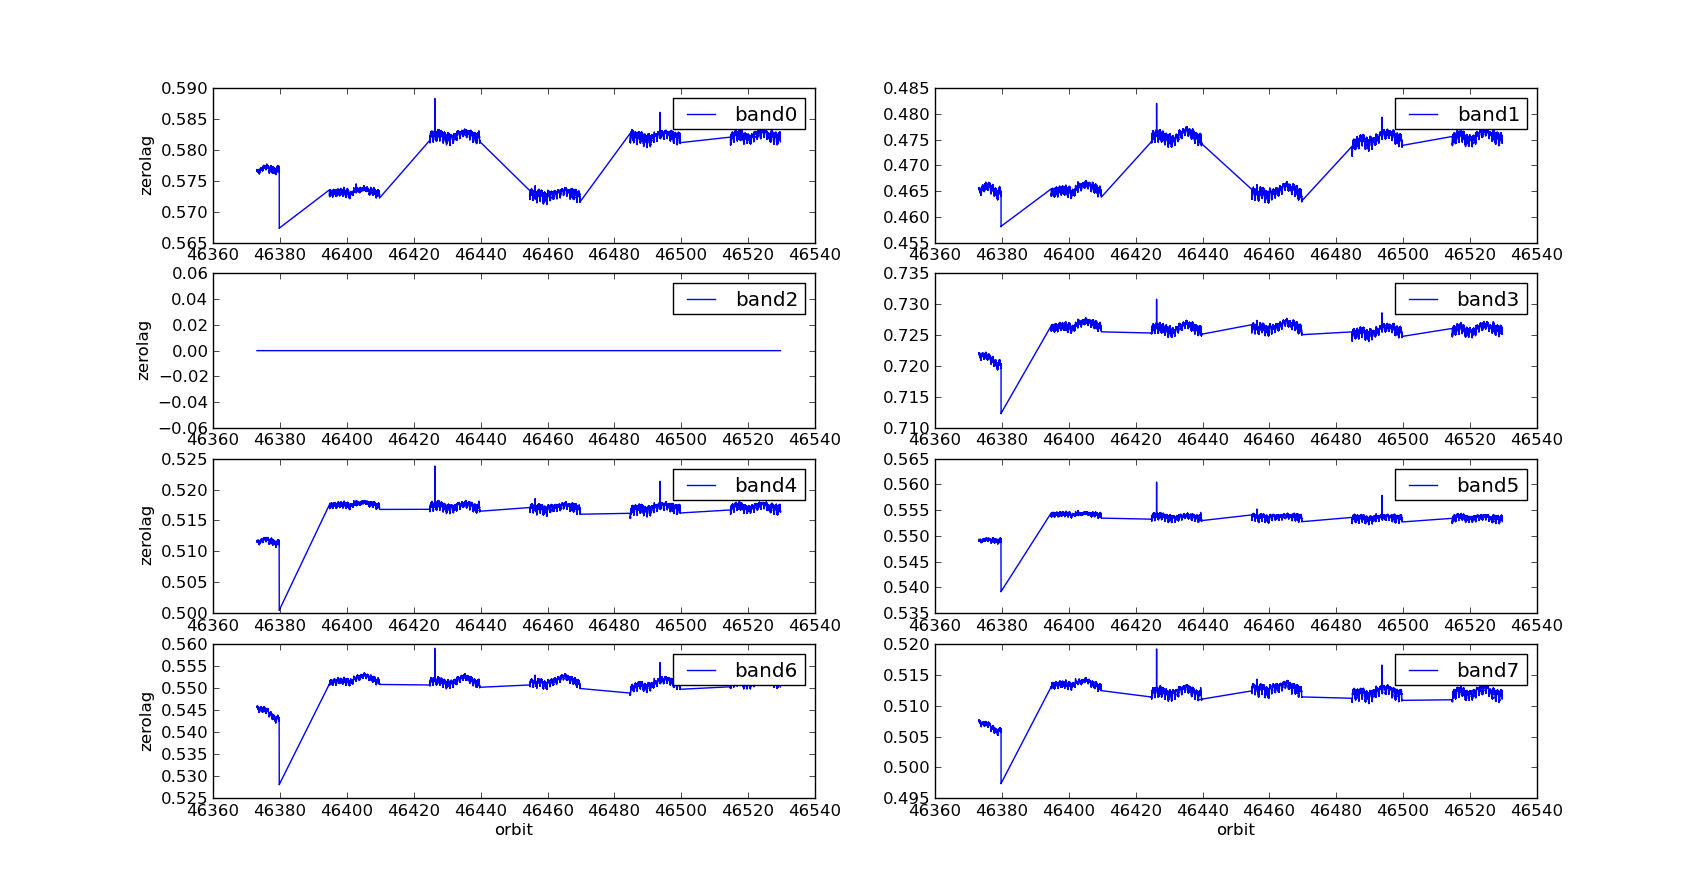
\includegraphics[scale=0.35]{ac2zerolag.png}\\
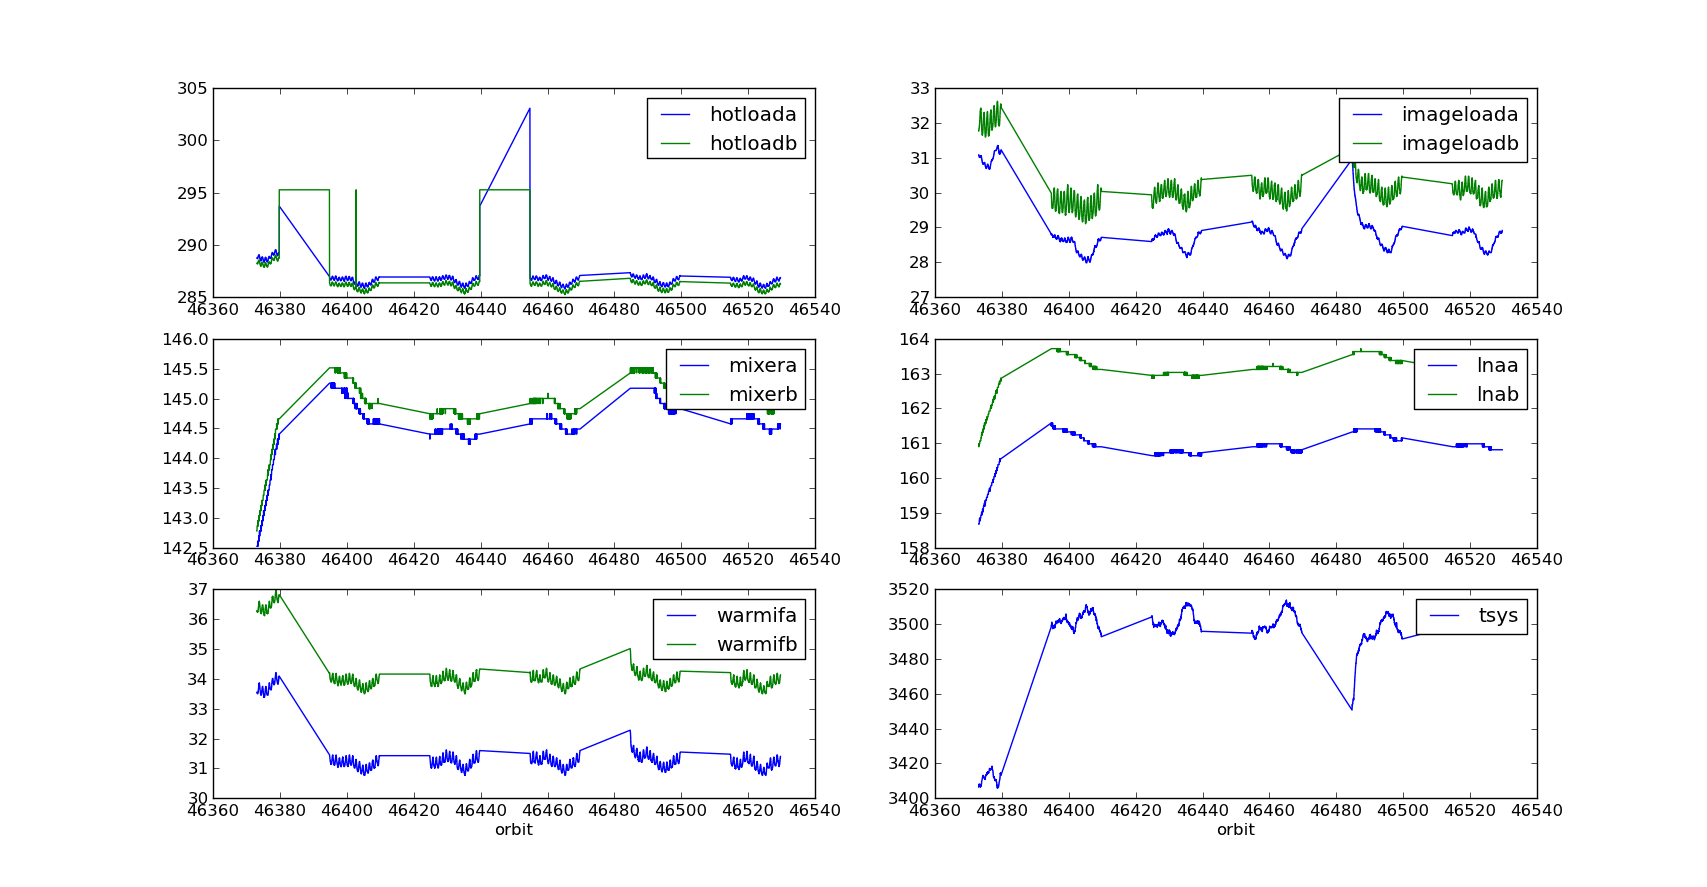
\includegraphics[scale=0.35]{ac2temp.png}\\
\caption{The upper panels show zerolags for the sky beam from AC2 
(stratospheric 1 mode)
for around 100 orbits. The lower panels show temperature information.}
\label{fig:study1ac2a}
\end{figure}

\begin{figure}[!t]
\centering
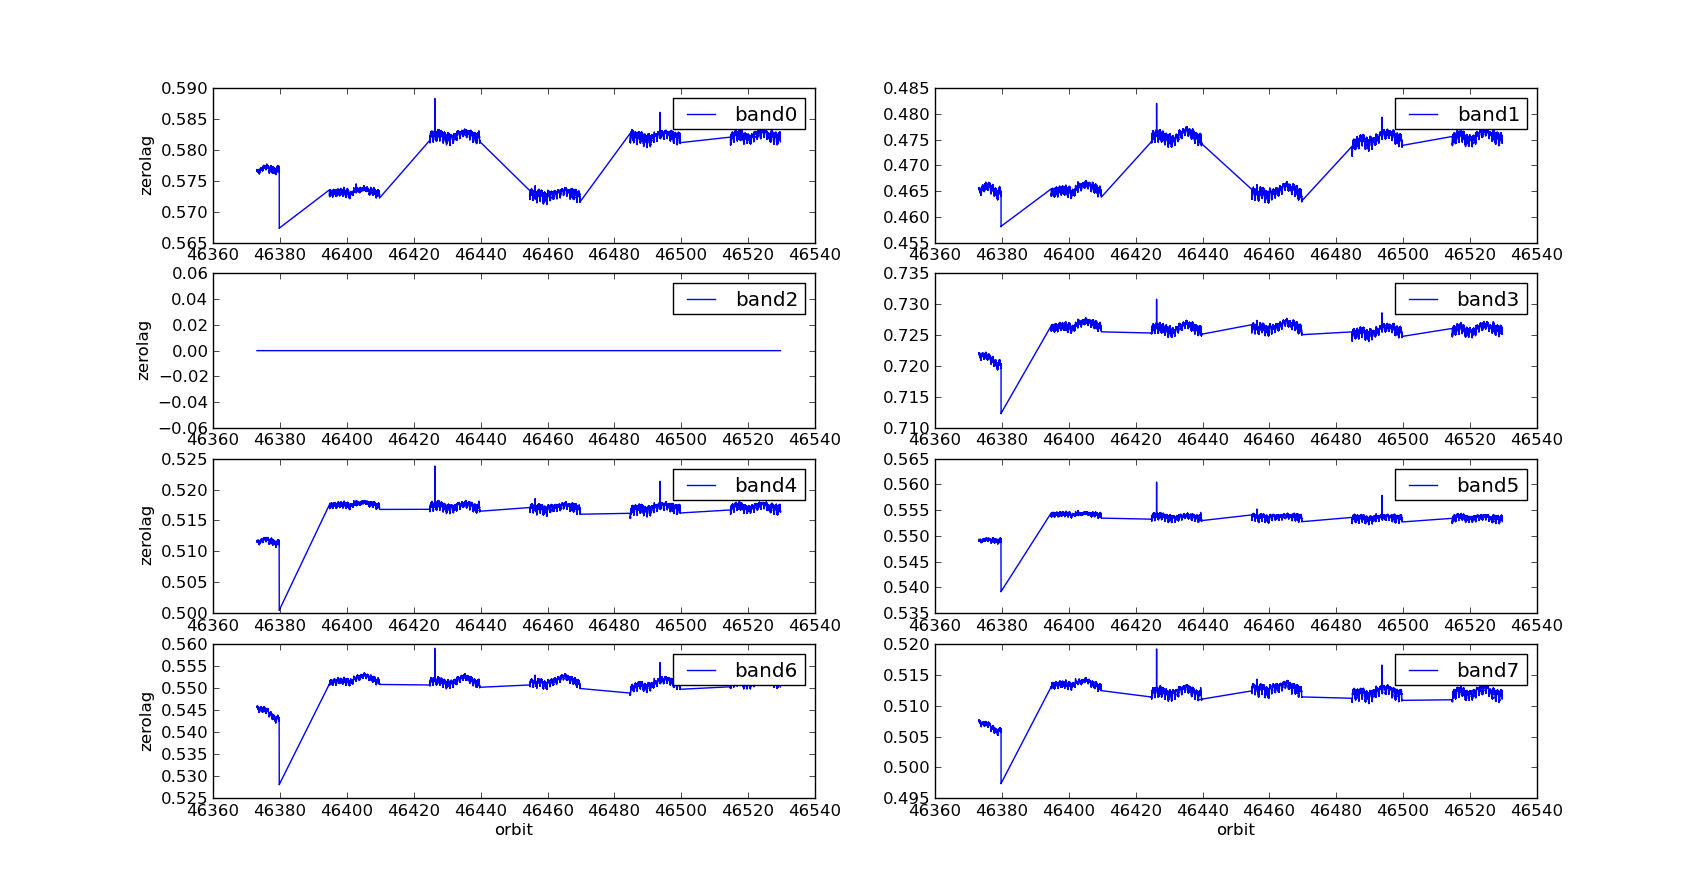
\includegraphics[scale=0.35]{ac2zerolag.png}\\
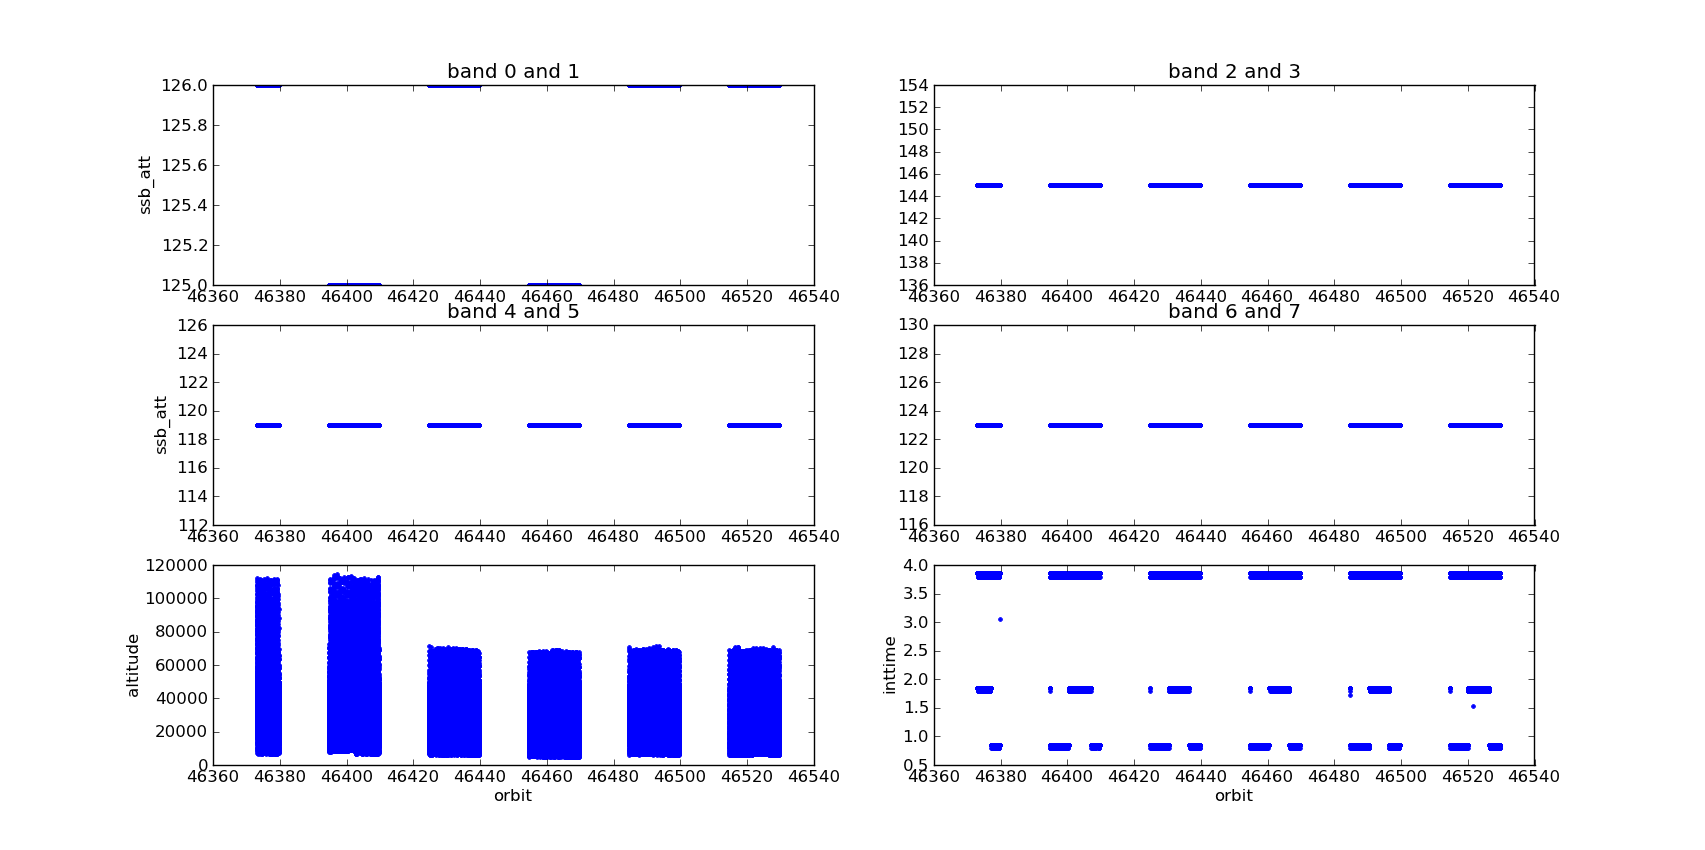
\includegraphics[scale=0.35]{ac2ssbatt.png}\\
\caption{The upper panels show zerolags for the sky beam from AC2 
(stratospheric 1 mode)
ssb-attenuators settings, altitudes, and integration times
matching Fig.~\ref{fig:study1ac2a}.}
\label{fig:ac2b}
\end{figure}

\begin{figure}[!t]
\centering
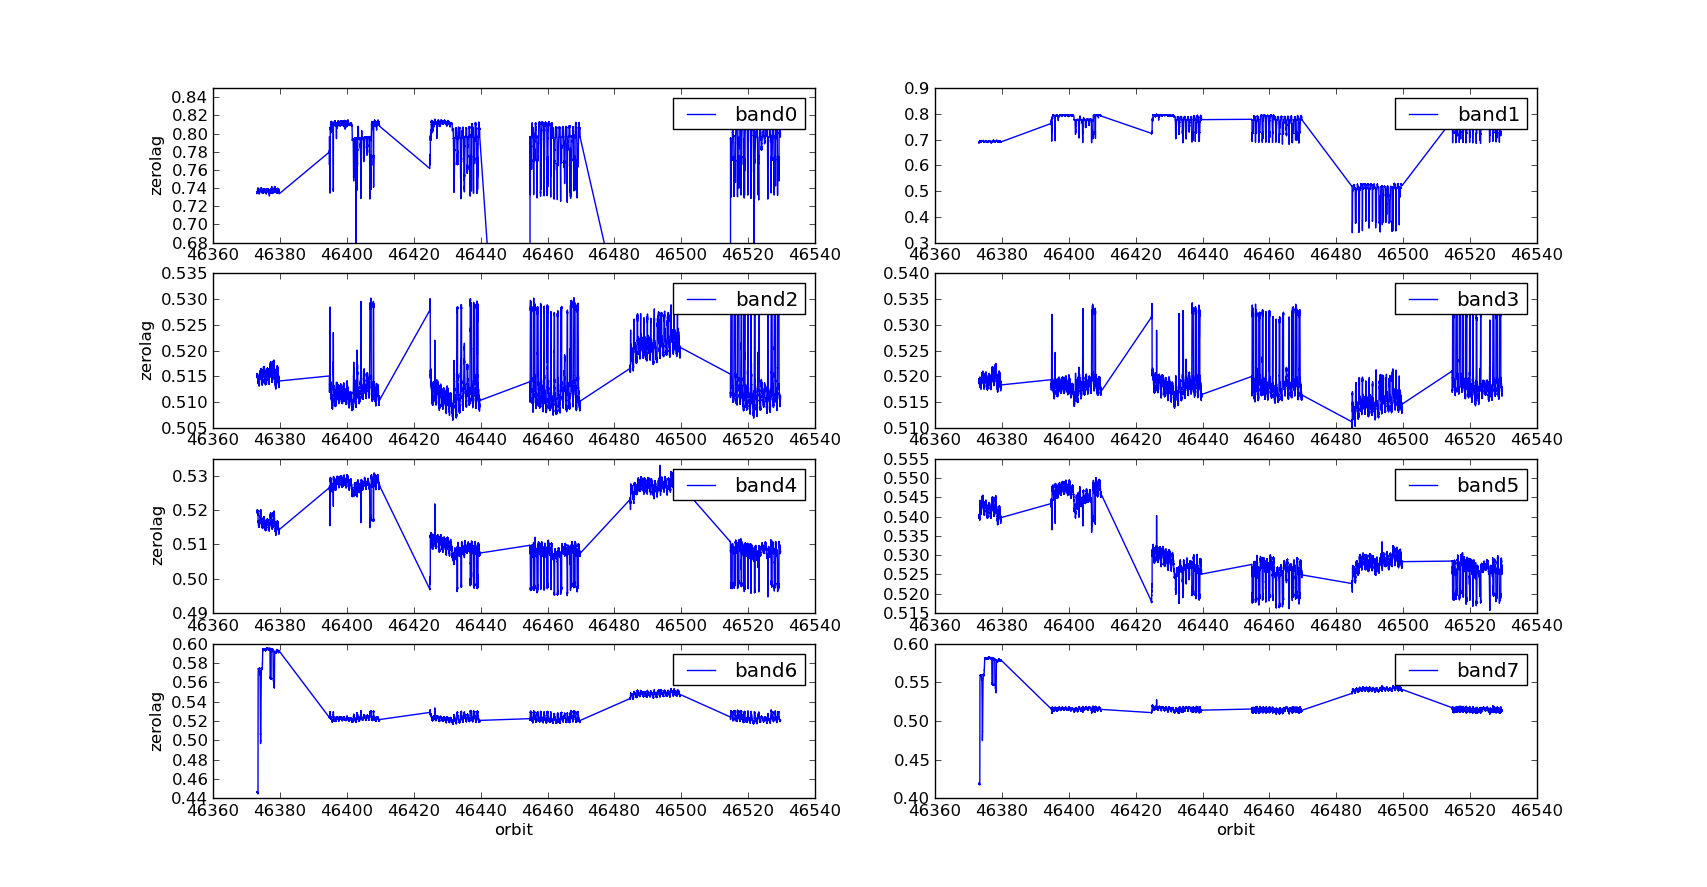
\includegraphics[scale=0.35]{ac1zerolag.png}\\
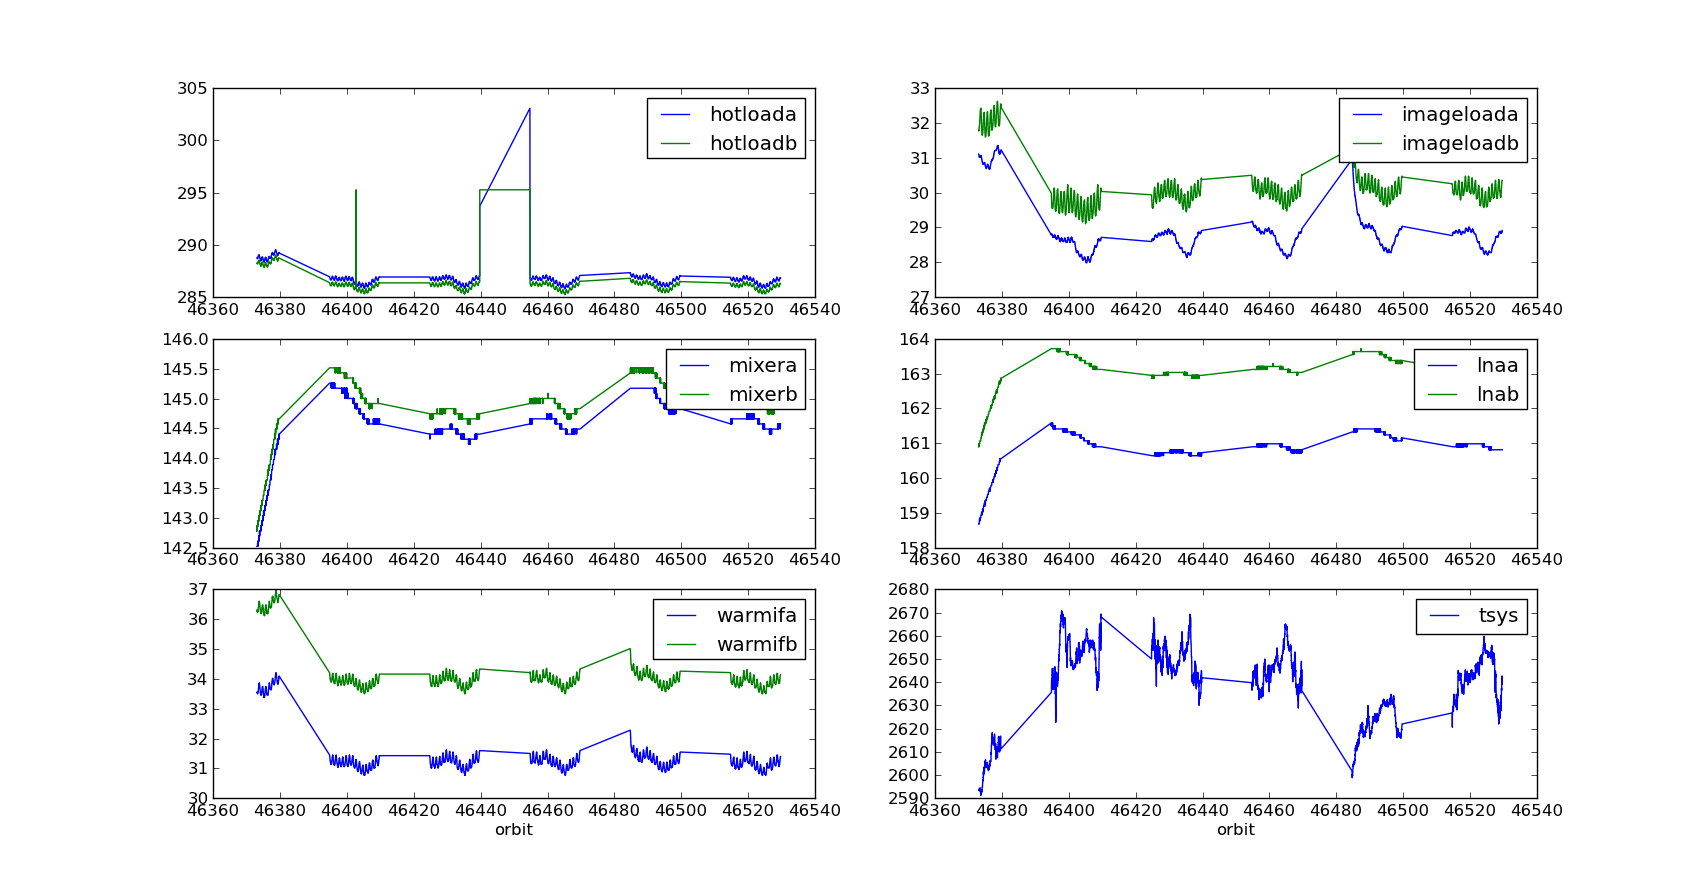
\includegraphics[scale=0.35]{ac1temp.png}
\caption{The upper panels show zerolags for the sky beam from AC1 
(stratospheric 2 mode)
for around 100 orbits. The lower panels show temperature information.}
\label{fig:study1ac1a}
\end{figure}

\begin{figure}[!t]
\centering
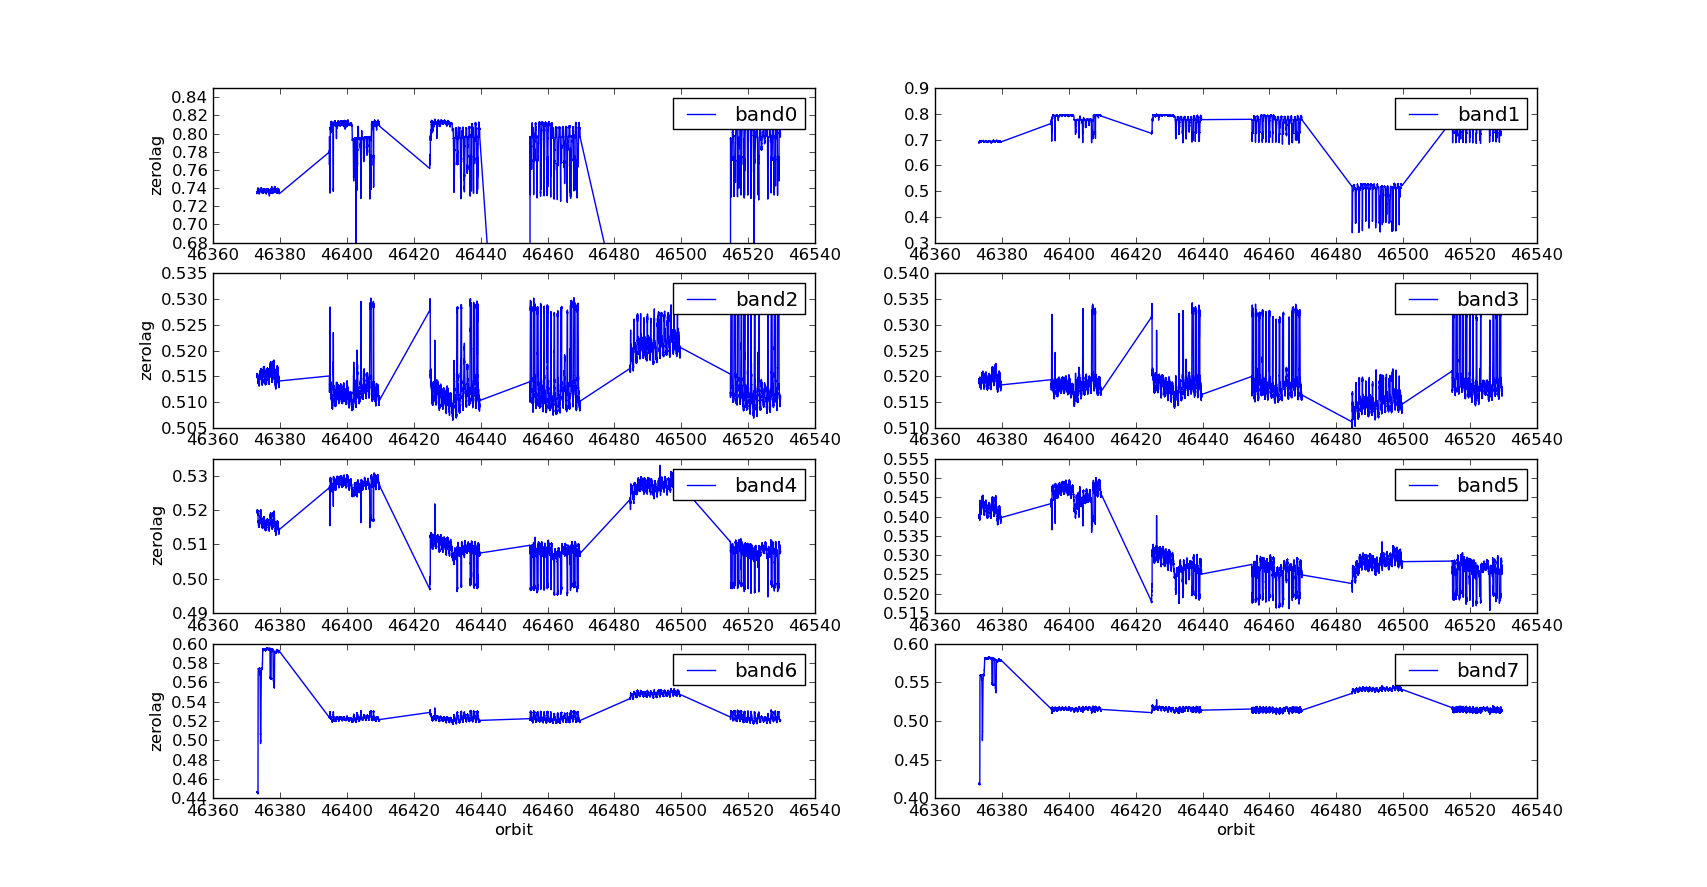
\includegraphics[scale=0.35]{ac1zerolag.png}\\
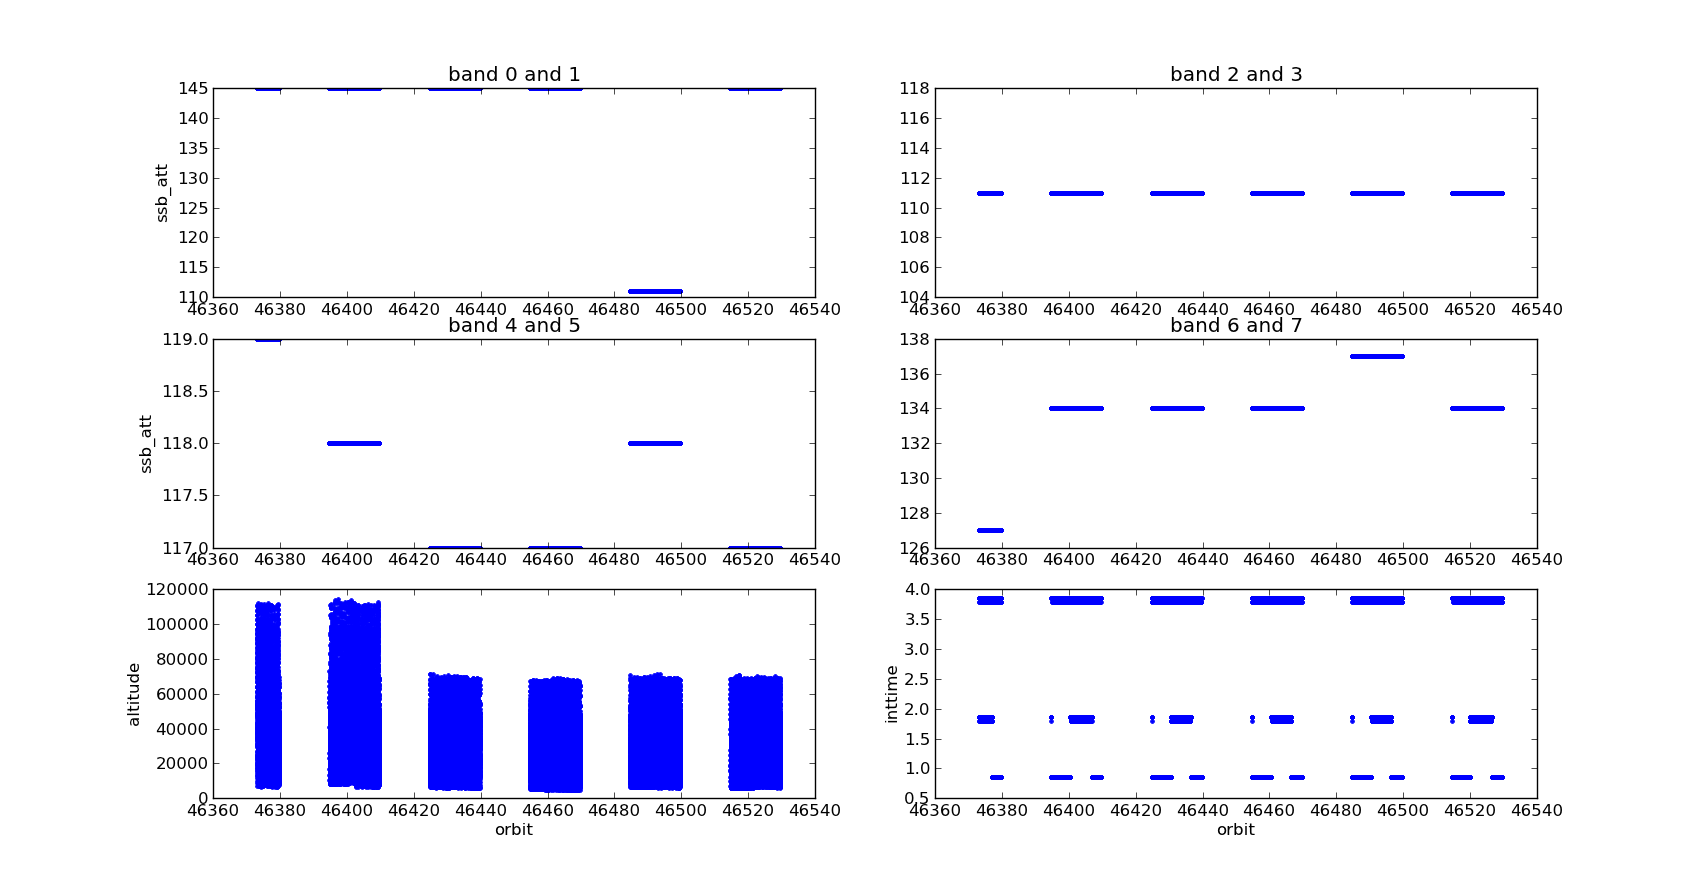
\includegraphics[scale=0.35]{ac1ssbatt.png}\\
\caption{ssb-attenuators settings, altitudes, and integration times
matching Fig.~\ref{fig:study1ac1a}.}
\label{fig:study1ac1b}
\end{figure}

%%%%%
\begin{figure}[!t]
\centering
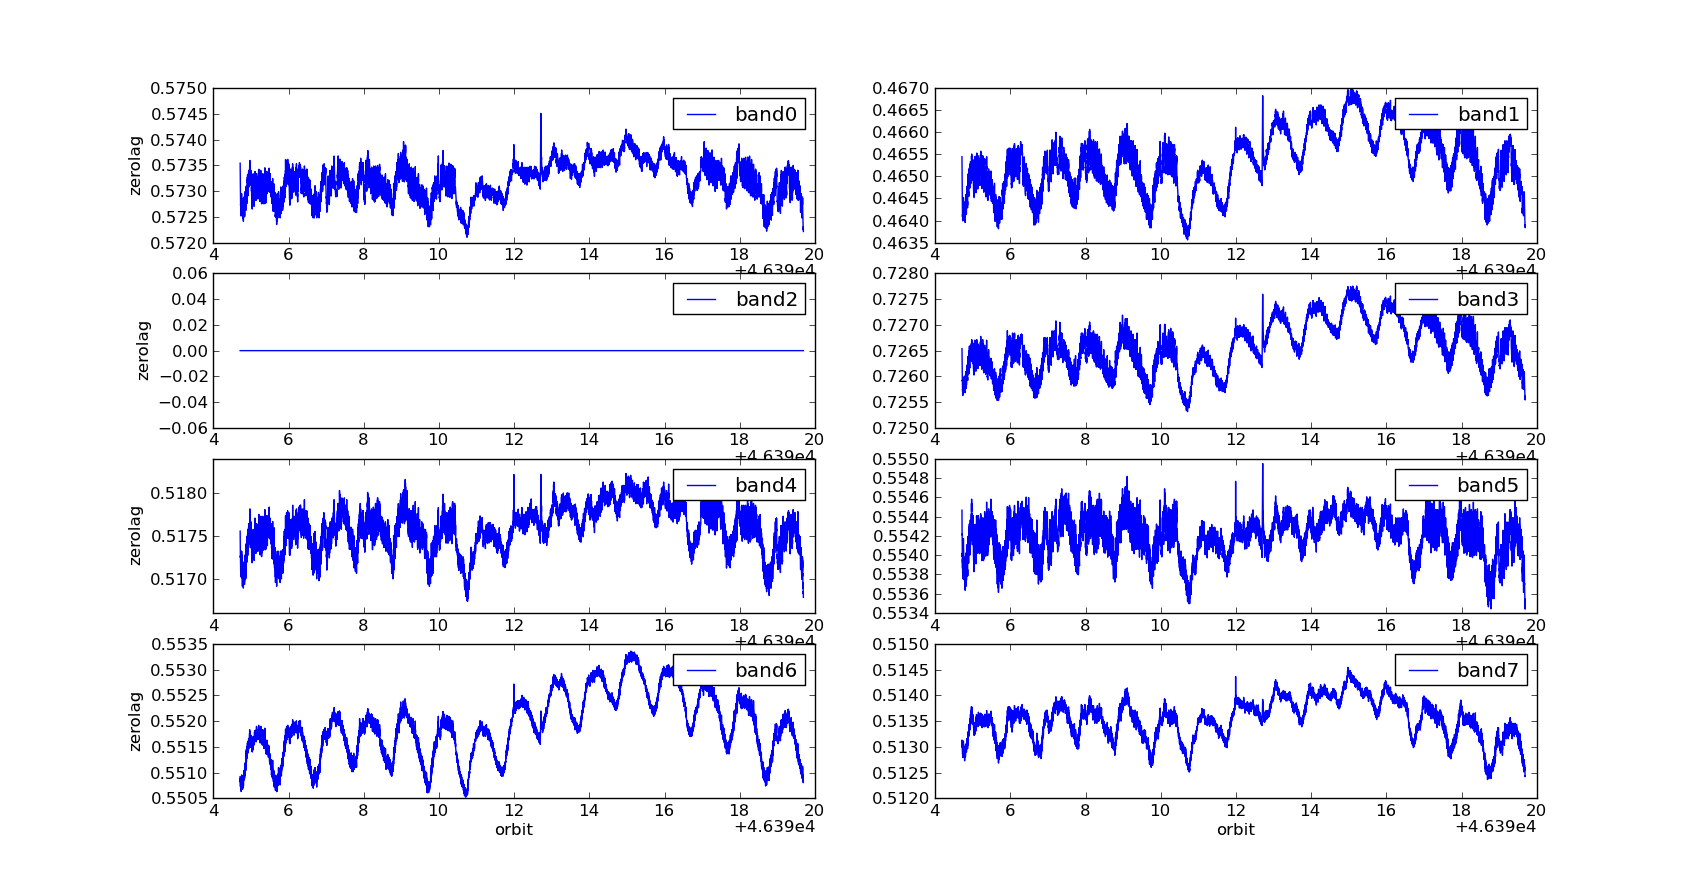
\includegraphics[scale=0.35]{ac2zerolag20orbits.png}\\
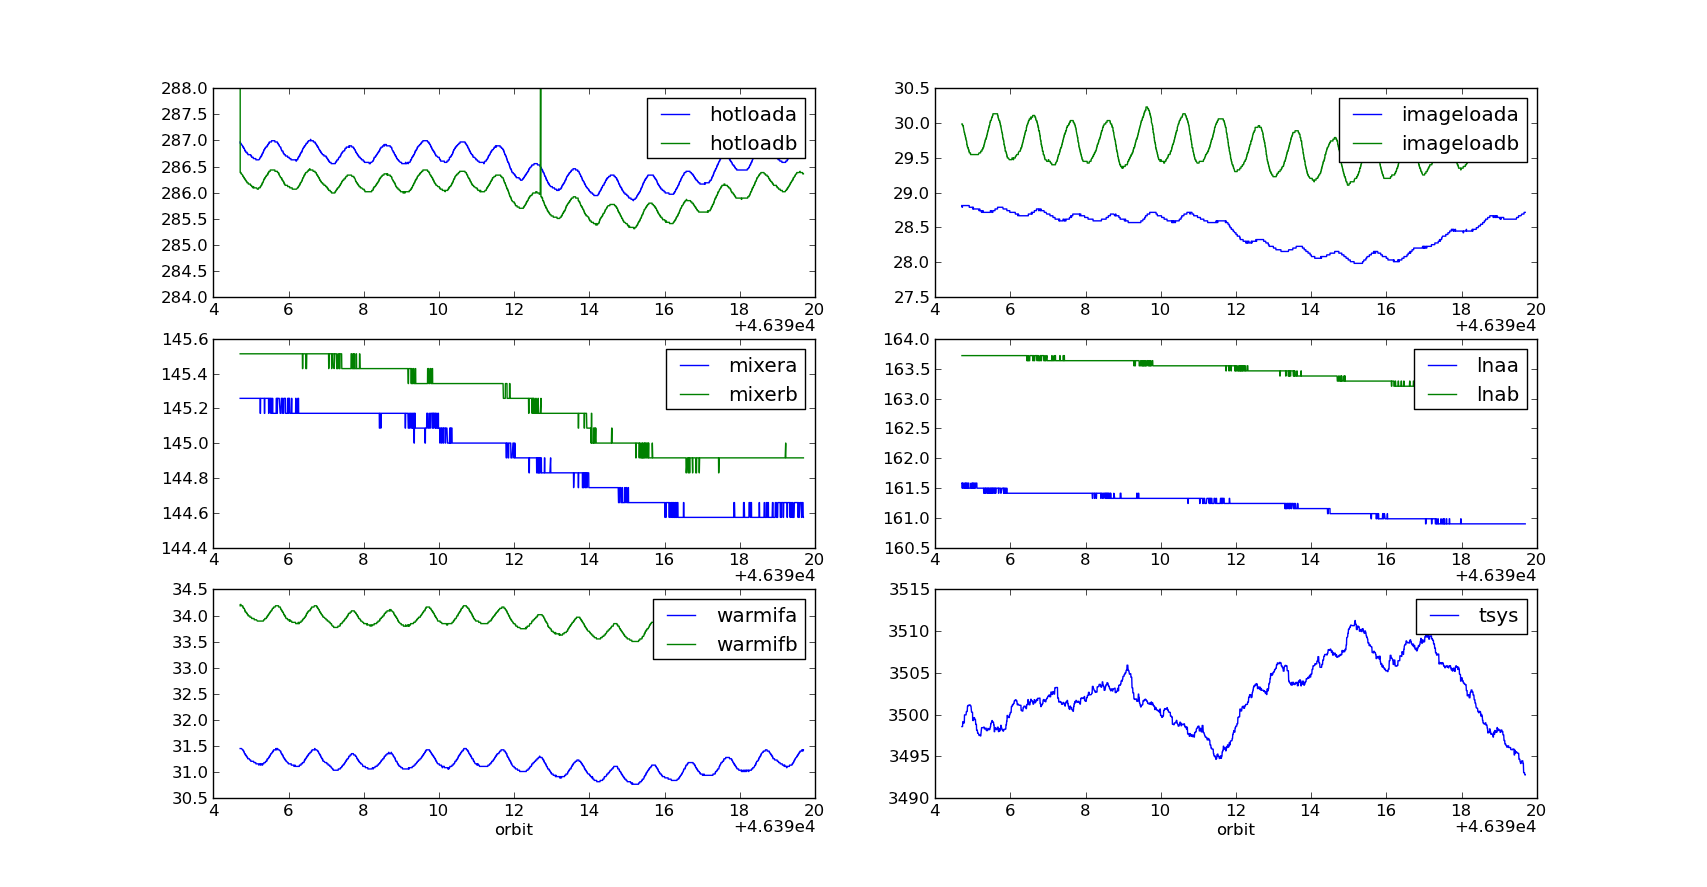
\includegraphics[scale=0.35]{ac2temp20orbits.png}\\
\caption{The upper panels show zerolags for the sky beam from AC2 
(stratospheric 1 mode)
for around 20 orbits. The lower panels show temperature information.}
\label{fig:study1ac2c}
\end{figure}

\begin{figure}[!t]
\centering
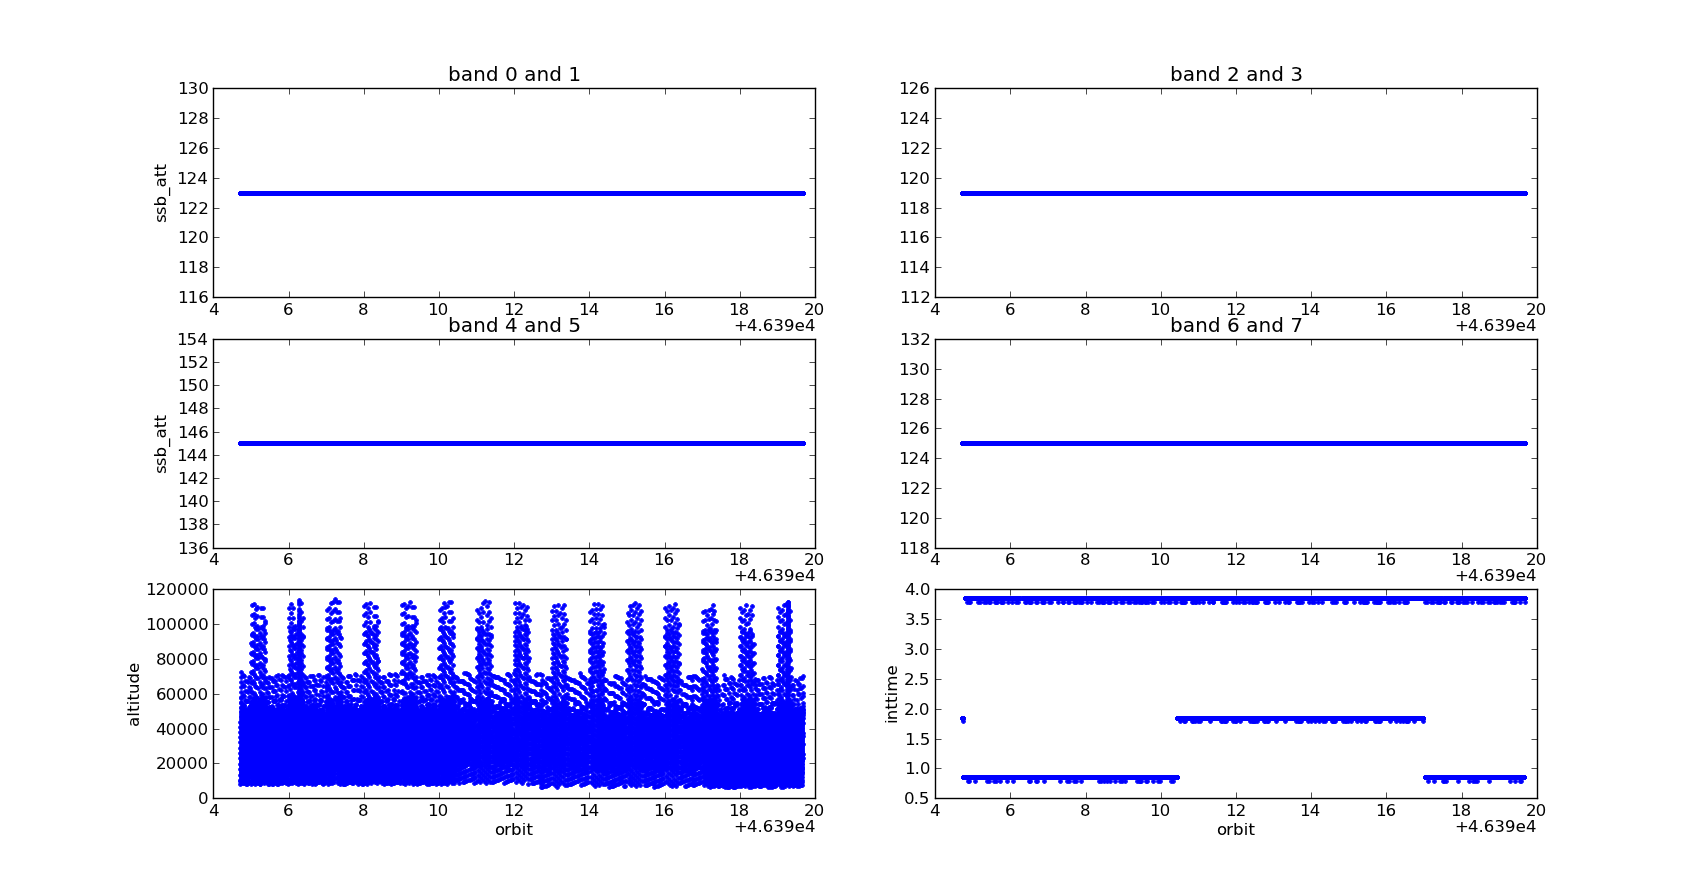
\includegraphics[scale=0.35]{ac2ssbatt20orbits.png}
\caption{ssb-attenuators settings, altitudes, and integration times
matching Fig.~\ref{fig:study1ac2c}.}
\label{fig:study1ac2d}
\end{figure}

\begin{figure}[!t]
\centering
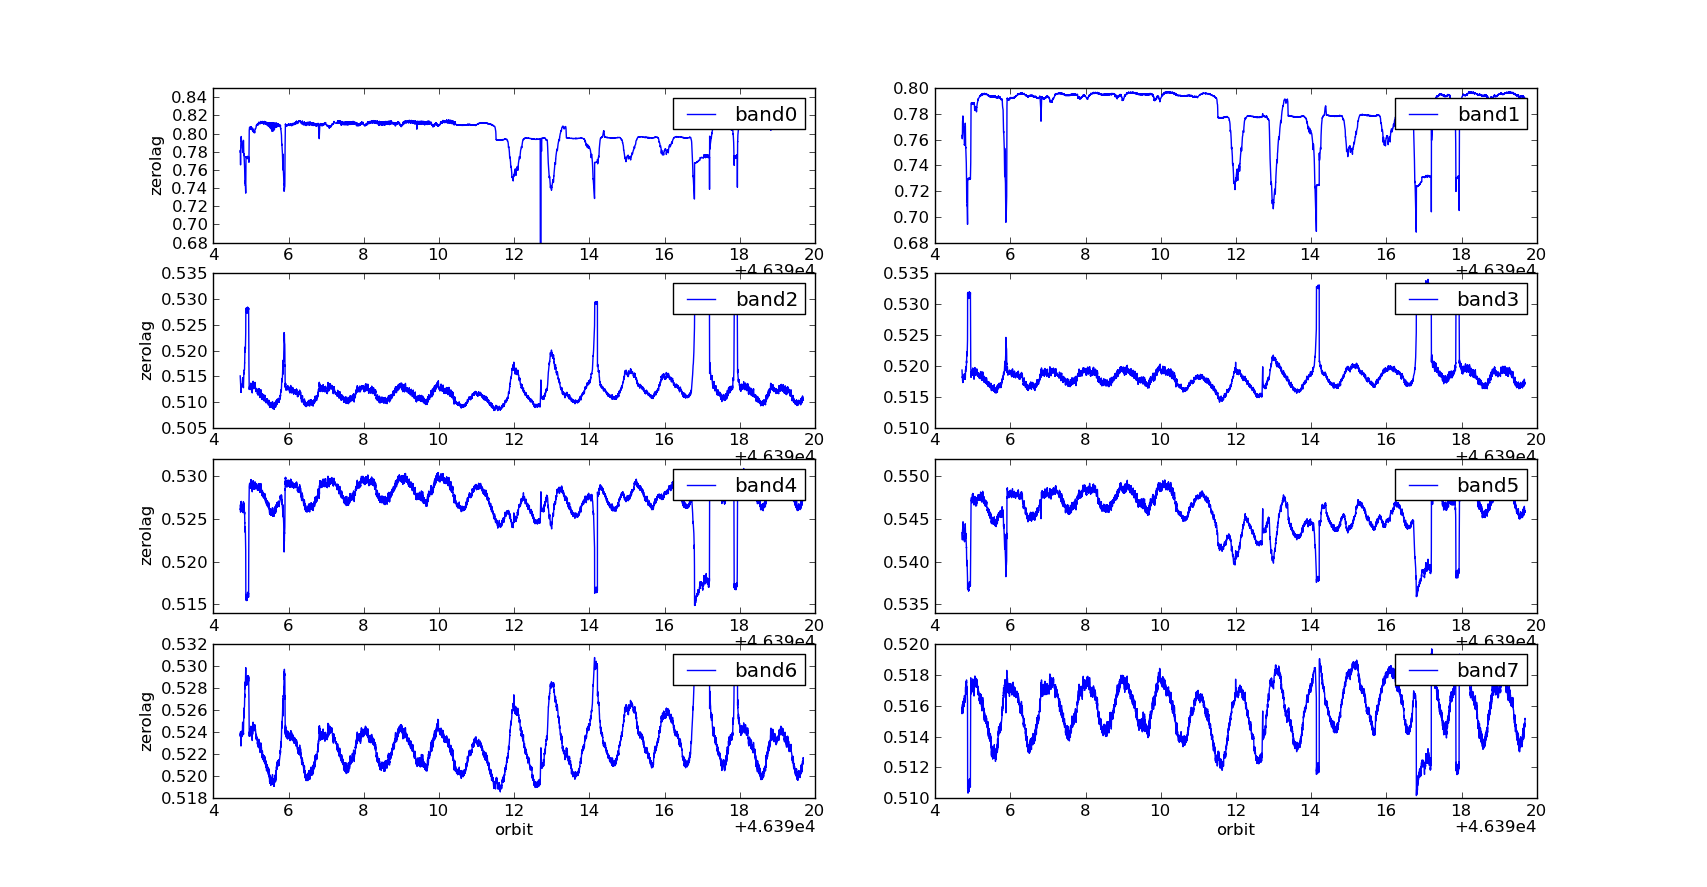
\includegraphics[scale=0.35]{ac1zerolag20orbits.png}\\
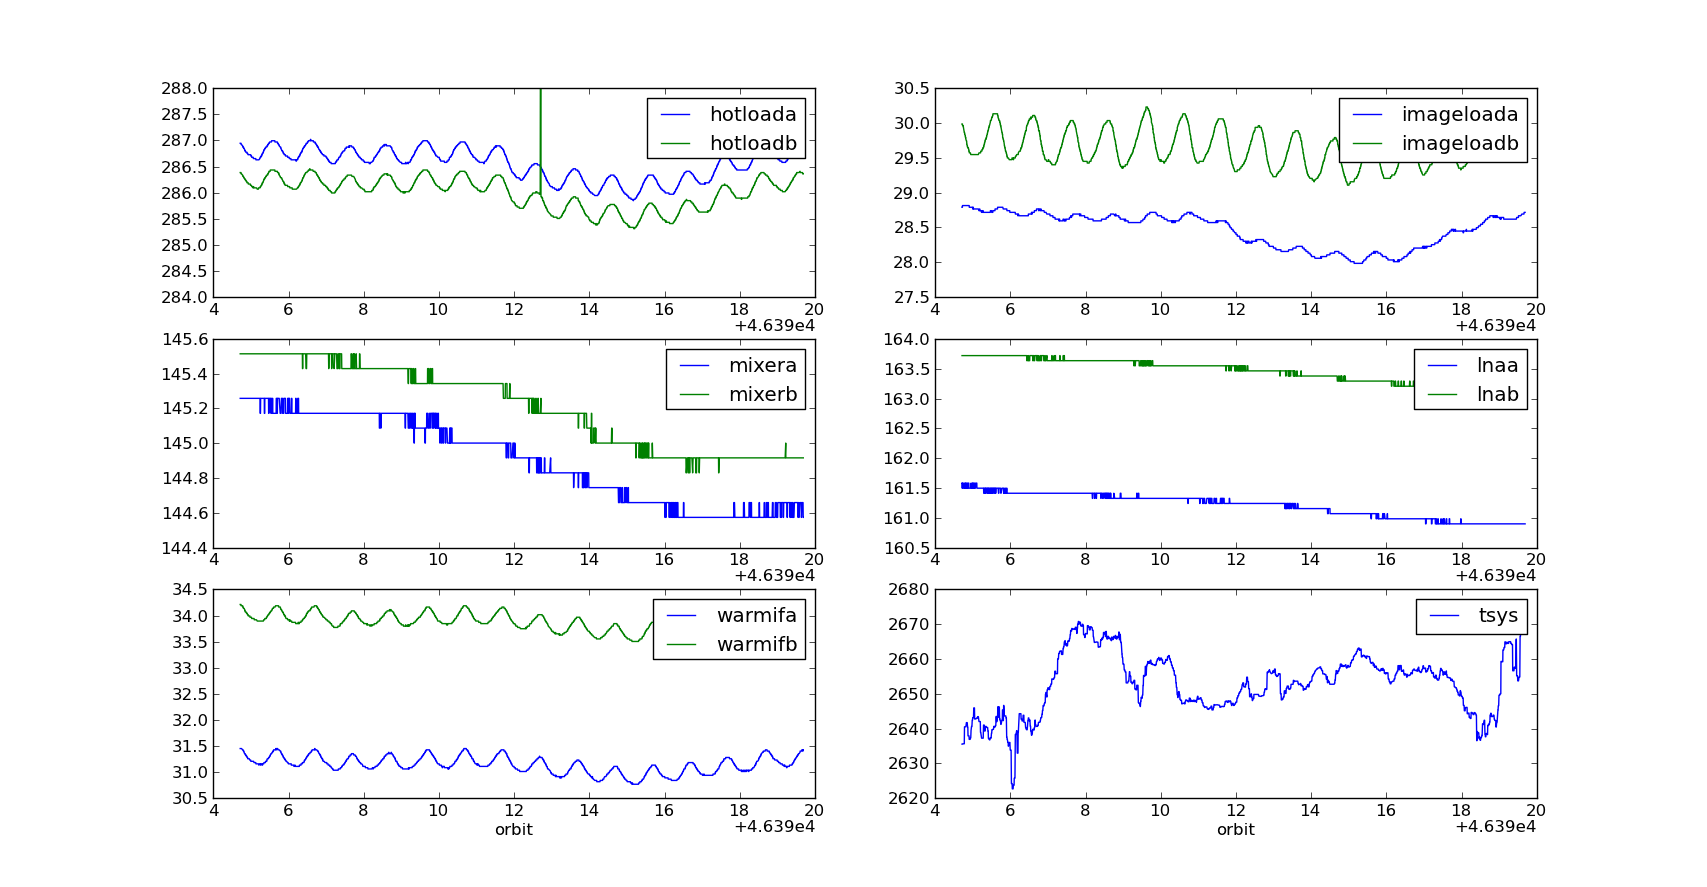
\includegraphics[scale=0.35]{ac1temp20orbits.png}
\caption{The upper panels show zerolags for the sky beam from AC1 
(stratospheric 2 mode)
for around 20 orbits. The lower panels show temperature information.}
\label{fig:study1ac1c}
\end{figure}

\begin{figure}[!t]
\centering
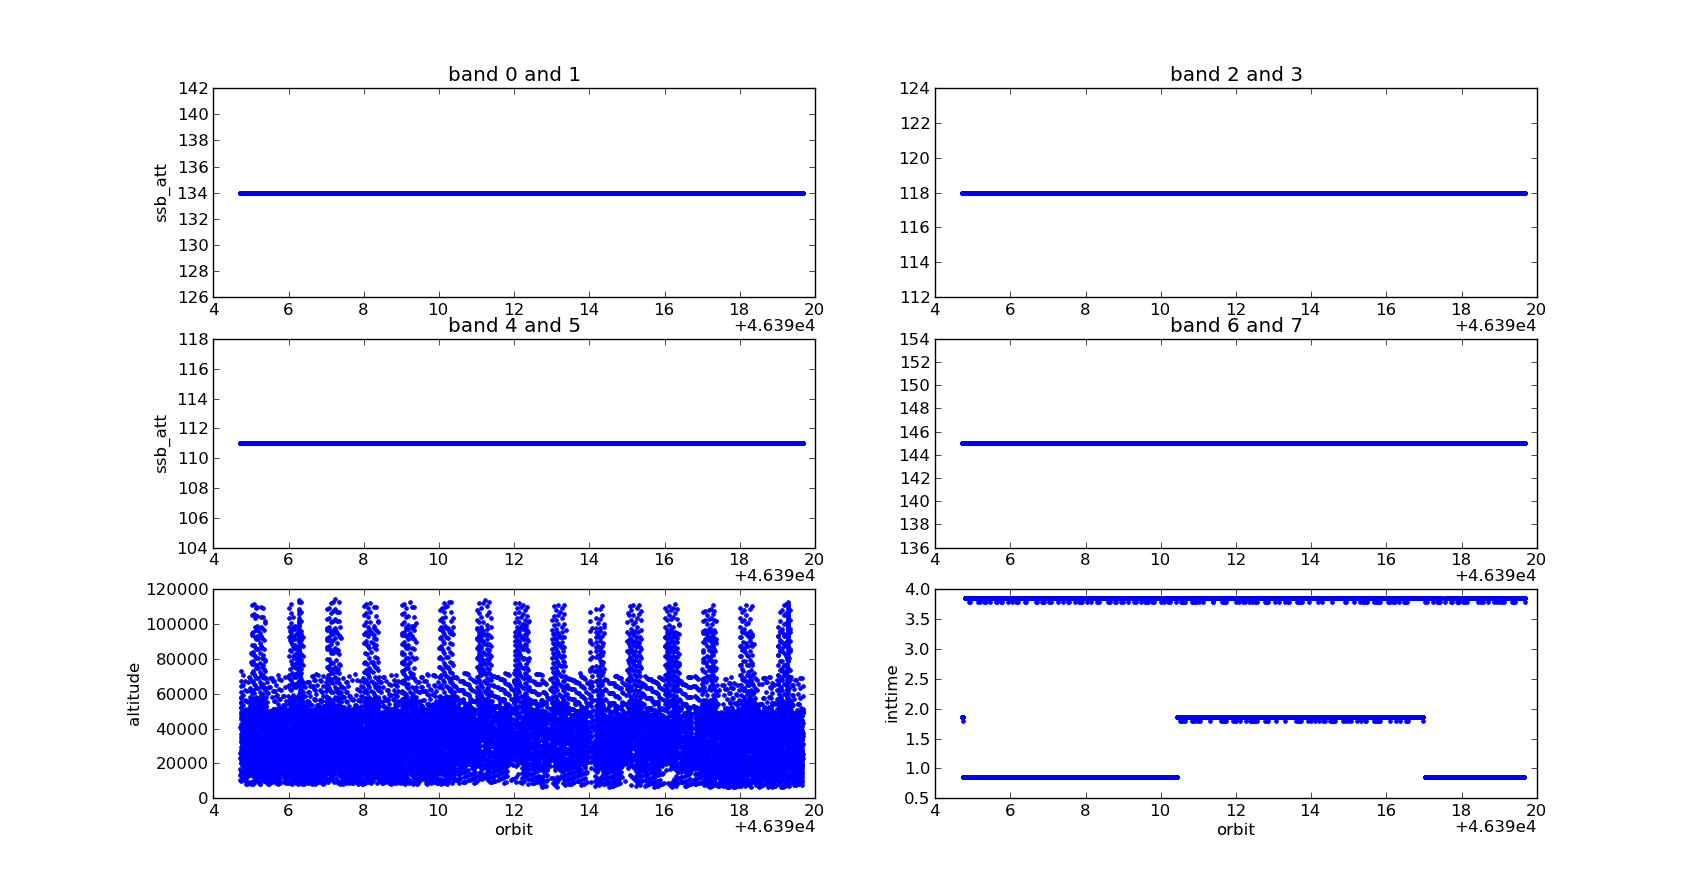
\includegraphics[scale=0.35]{ac1ssbatt20orbits.png}
\caption{ssb-attenuators settings, altitudes, and integration times
matching Fig.~\ref{fig:study1ac1c}.}
\label{fig:study1ac1d}
\end{figure}

We have earlier seen that we have variations in the zerolag
levels for the various bands of AC1 and AC2 that we want to
understand better. In the following figures zerolags
are plotted together with various temperature information
(more than we have shown earlier)
as function of orbit.
From Figures~\ref{fig:study1ac2a} and ~\ref{fig:study1ac1a},
which shows zerolags from AC2 and AC1 for around 100 orbits,
we can see that AC2 is more stable than AC1. 
The zerolgas of AC2 seems to be fairly stable for each period
of observation, even though the level can differ between different
periods (see band 0 and band 1 in Figure~\ref{fig:study1ac2a}).
This latter variation can not easily be explained by the temperature
information we have.

From Figures~\ref{fig:study1ac2c} and ~\ref{fig:study1ac1c}
which show zerolags from AC2 and AC1 for around 20 orbits
(a period where the observation modes were not changed),
it can be seen that AC2 zerolags are correlated to various
temperatures. When temperature is relatively high zerolags are
relatively low and vice versa.
Even AC1 zerolags show this pattern, but for some periods of time
the levels of zerolags changes in a way that we do not see from AC2.
Figure~\ref{fig:study1ac1c} shows also that the level of zerolag of each band 
of AC1 can occasionally change. 

\clearpage
\newpage
\section{High altitude spectra}
\begin{figure}[!t]
\centering
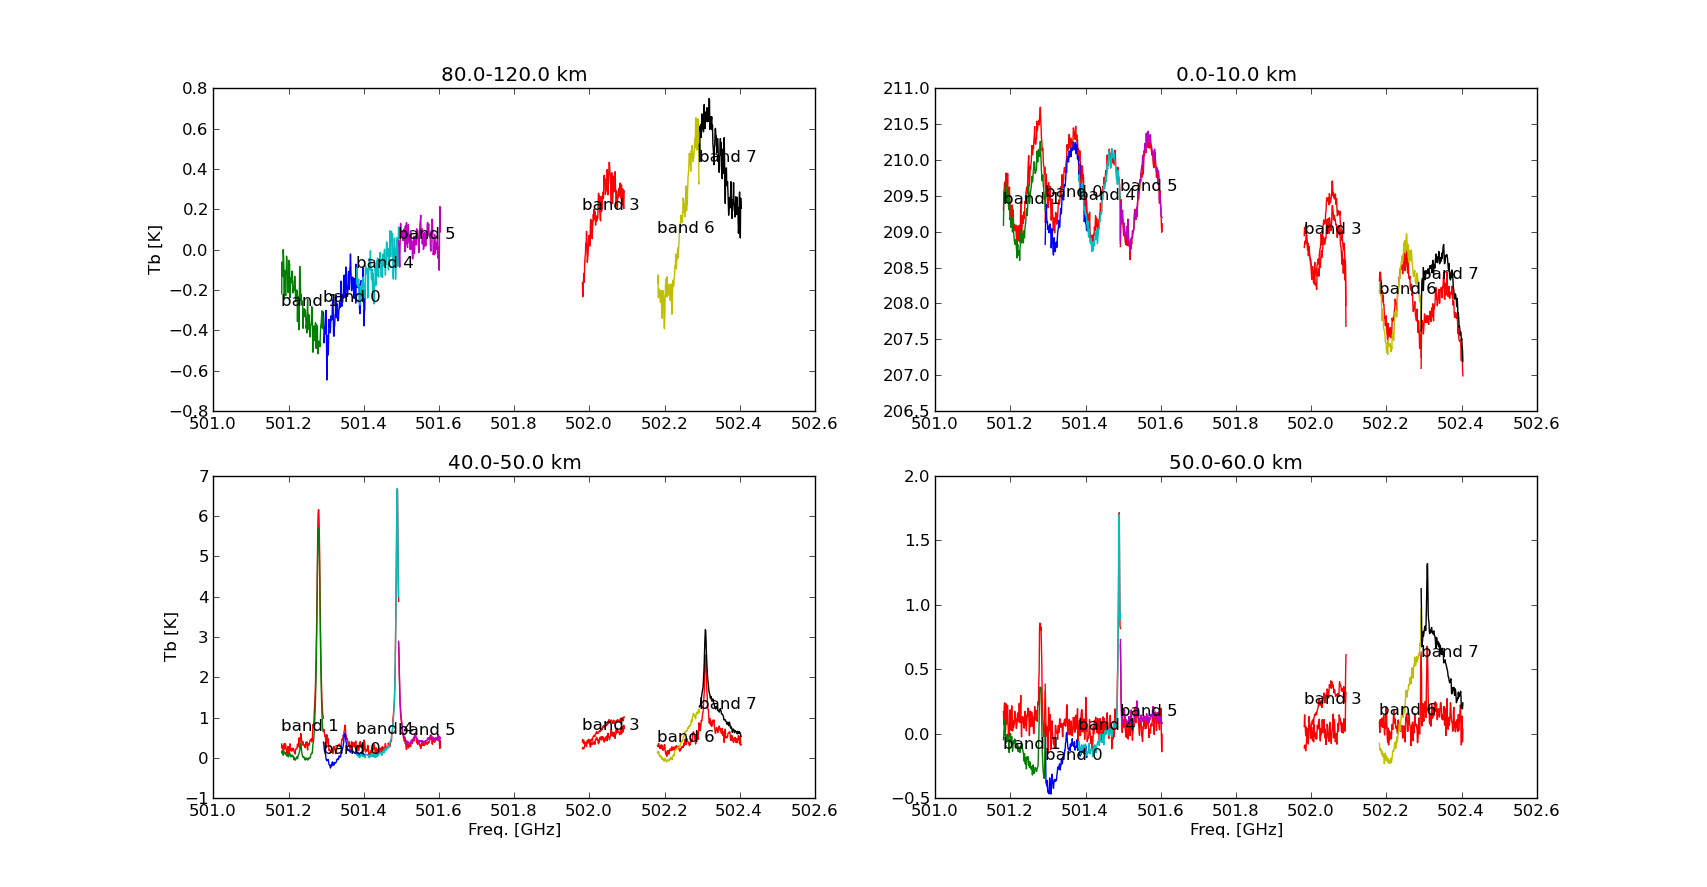
\includegraphics[scale=0.35]{ac2corr.png}
\caption{Calibrated data from AC2. The upper left panel shows
the median of measurents between 80-120 km. The other panels contain
both the mean of calibrated spectra between the heights in the title
of panels, and a spectrum (red) where the median of measurents between 80-120 km
has been subtracted. }
\label{fig:study1ac2corr}
\end{figure}


\begin{figure}[!t]
\centering
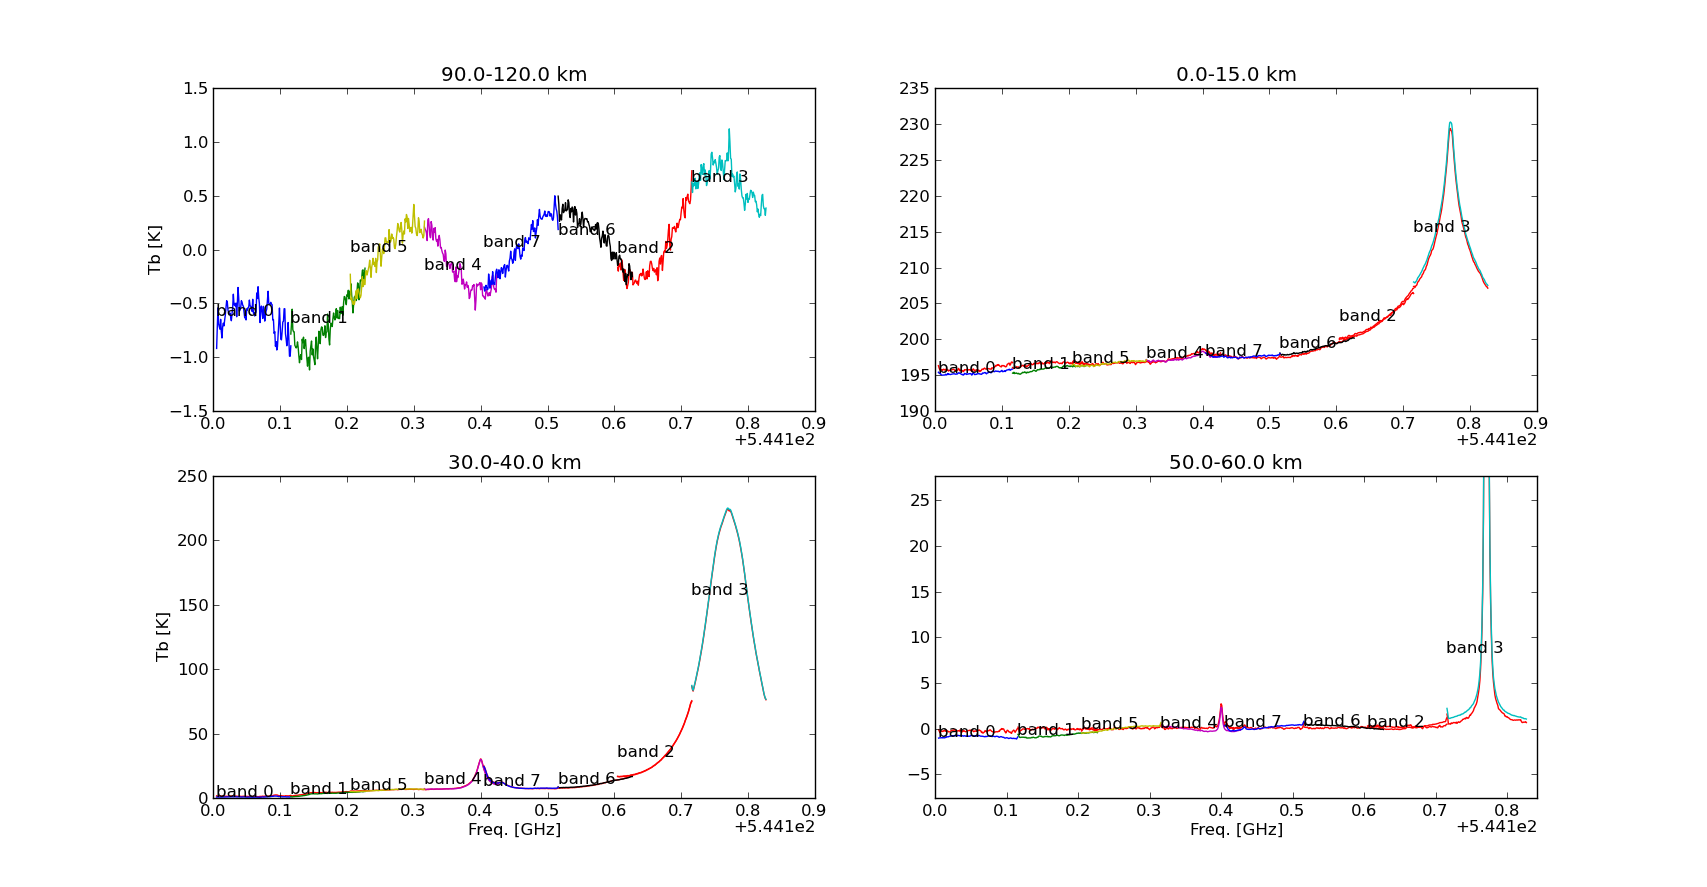
\includegraphics[scale=0.35]{ac1corr.png}
\caption{Calibrated data from AC2. The upper left panel shows
the median of measurents between 90-120 km. The other panels contain
both the mean of calibrated spectra between the heights in the title
of panels, and a spectrum (red) where the median of measurents between 90-120 km
has been subtracted.}
\label{fig:study1ac1corr}
\end{figure}
    
We know from earlier calibration versions of AC data from Odin-SMR
that high altitude spectrum, where we do not expect any spectral
feature, do contain a spectral feature. 

We have calibrated data from around 100 orbits where we have used
a slightly new calibration scheme (a \(\pm\)45 min window instead
of orbit-based calibration and a harder filtering of data). 
 
Figures~\ref{fig:study1ac2corr} and ~\ref{fig:study1ac1corr} show average
results from this calibration. From the upper left panels in
both figures it can be seen that average spectra still contains
spectral fetaures. The spectral fetaure from AC1 and AC2 looks
distincly different.
However, the spectral feature we also see from measurements
at lower altitudes (except from AC2 data at really low altitudes
where we see something else). The spectral feature at high altitudes
should have it's
origin in the antenna and the optics. The calibration scheme as it is
only corrects for this by a constant value (the mean of the mean
of high altitude spectra is close to zero).
Figures~\ref{fig:study1ac2corr} and ~\ref{fig:study1ac1corr} show that if we
subtract the ``high altitude signal'' from measurements from lower
altitudes these spectra looks more flat where it should.
Thus, the high spectral feature can be calibrated away (removed) 
as a frequency dependent tspill contribution.  

\section{Calibration of sky signals}
As a healty check of the calibration routine we have calibrated 
sky signals (not using the target sky signal in the calibration
process). Figures ~\ref{fig:study1ac2skysig} and ~\ref{fig:study1ac1skysig}
show time series of calibrated sky signals (mean of each band). 
On average the sky signal is close to 0 k, but occasionally
and specially
when zerolags timeseries looks ``strange'' the signal
can differ significantly from 0 K (see Figure~\ref{fig:study1ac1skysig}).

The calibrated sky signals before a target atmospheric signal 
can serve as a quality flag.


\begin{figure}[!t]
\centering
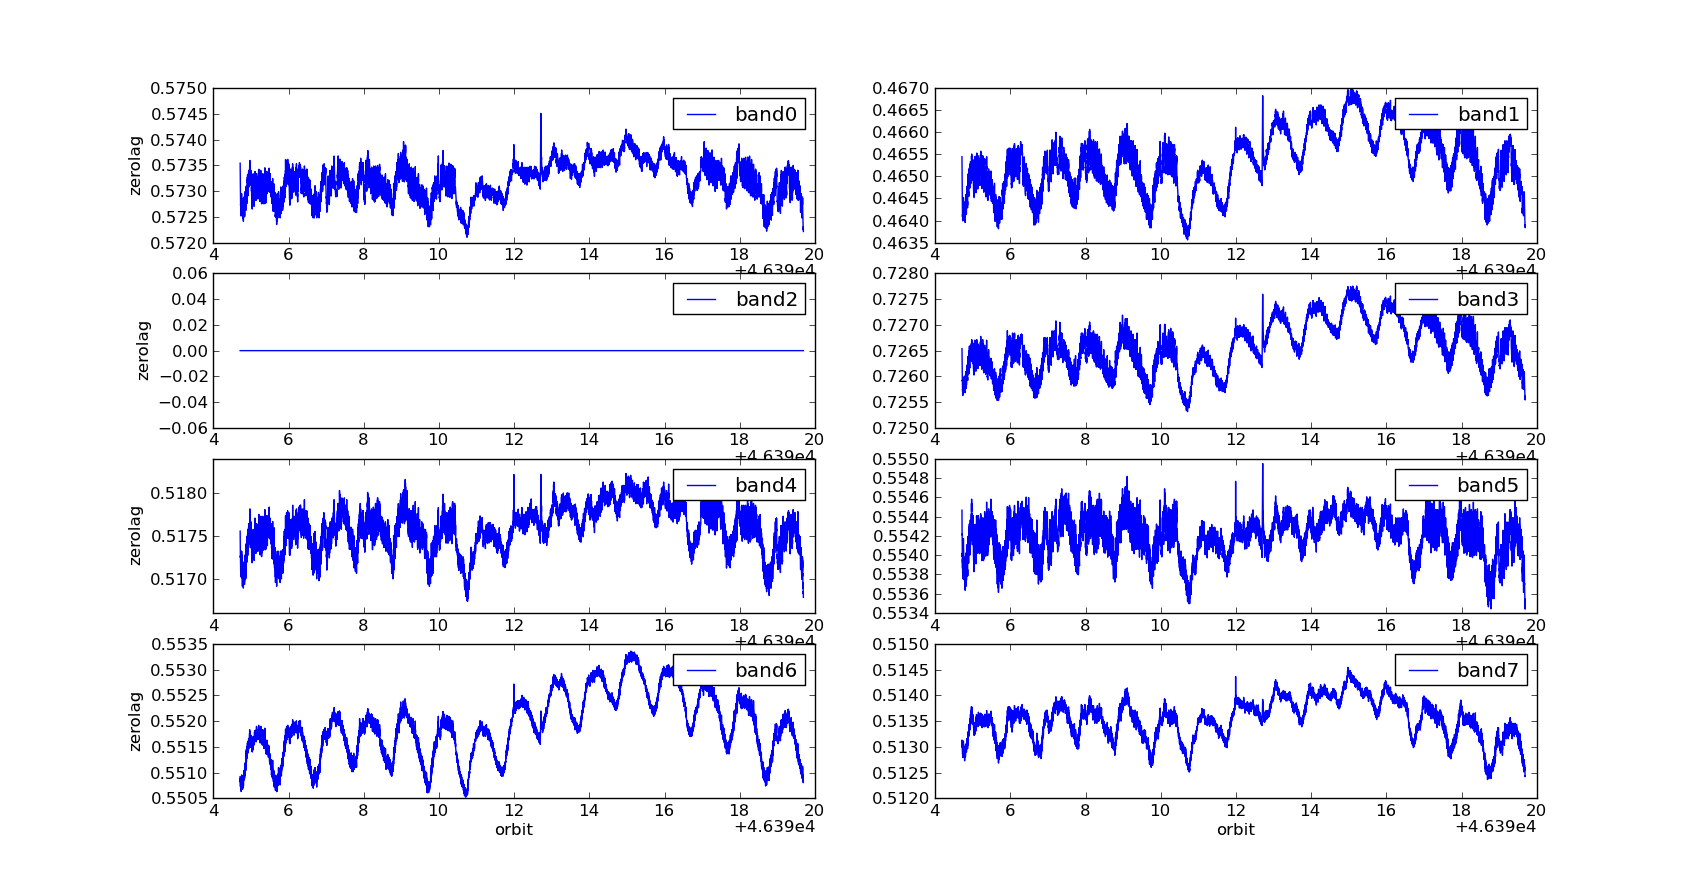
\includegraphics[scale=0.35]{ac2zerolag20orbits.png}
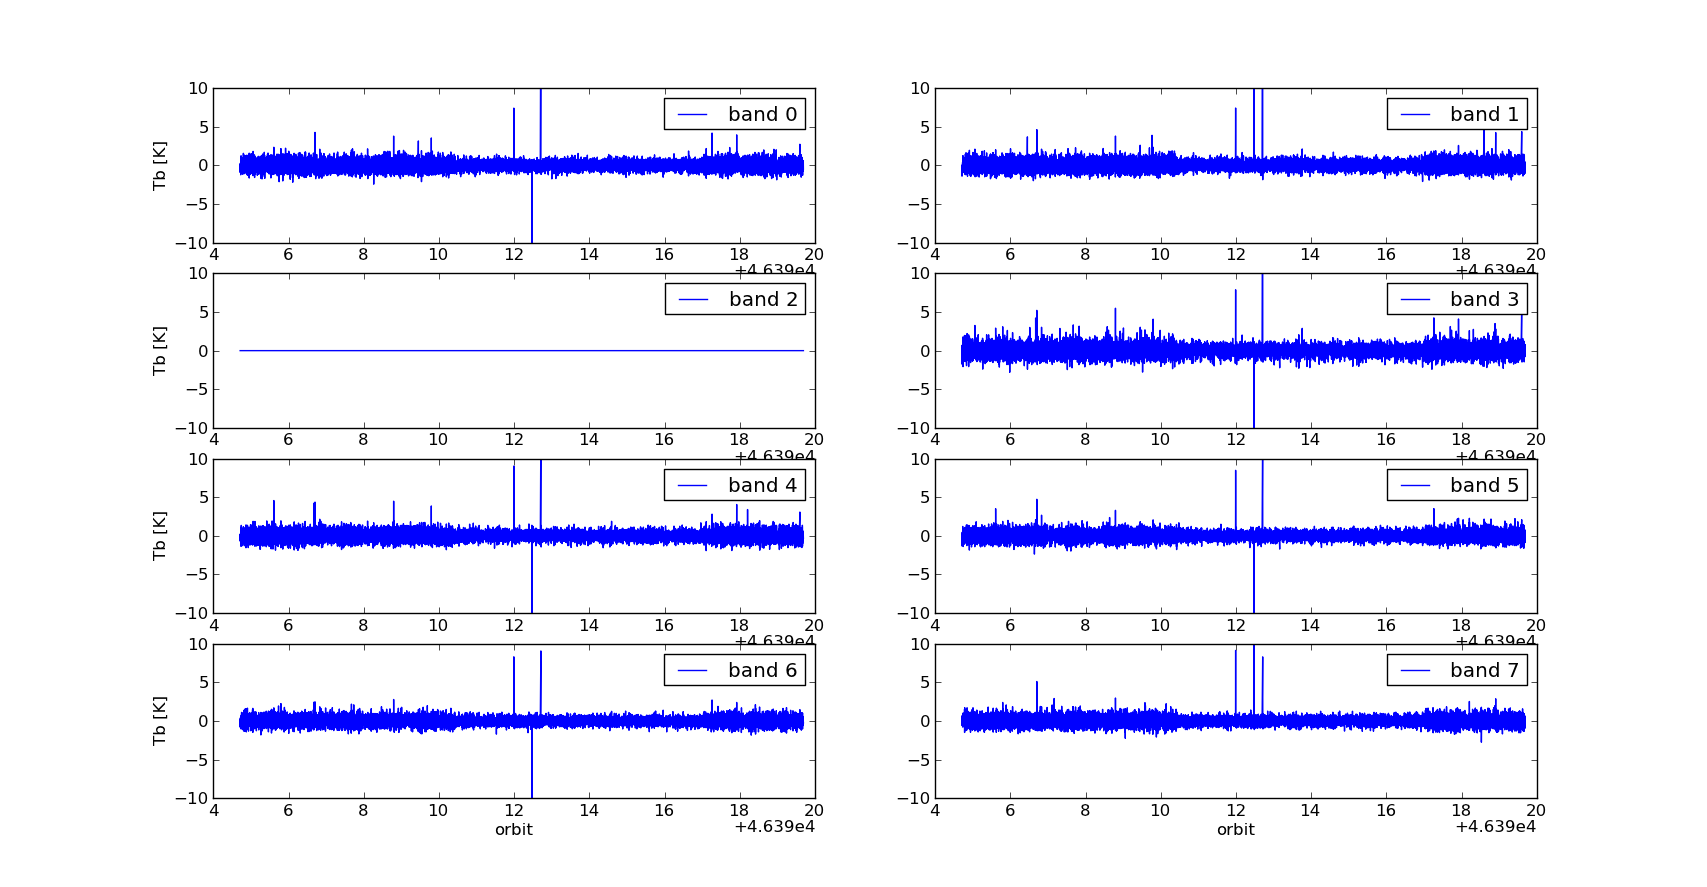
\includegraphics[scale=0.35]{ac2skysig.png}
\caption{The upper panels shows zerolags for AC2 (same as Figure~\ref{fig:study1ac2c}) and the lower panels shows the mean Tb of calibrated sky signals of each band.
}
\label{fig:study1ac2skysig}
\end{figure} 

\begin{figure}[!t]
\centering
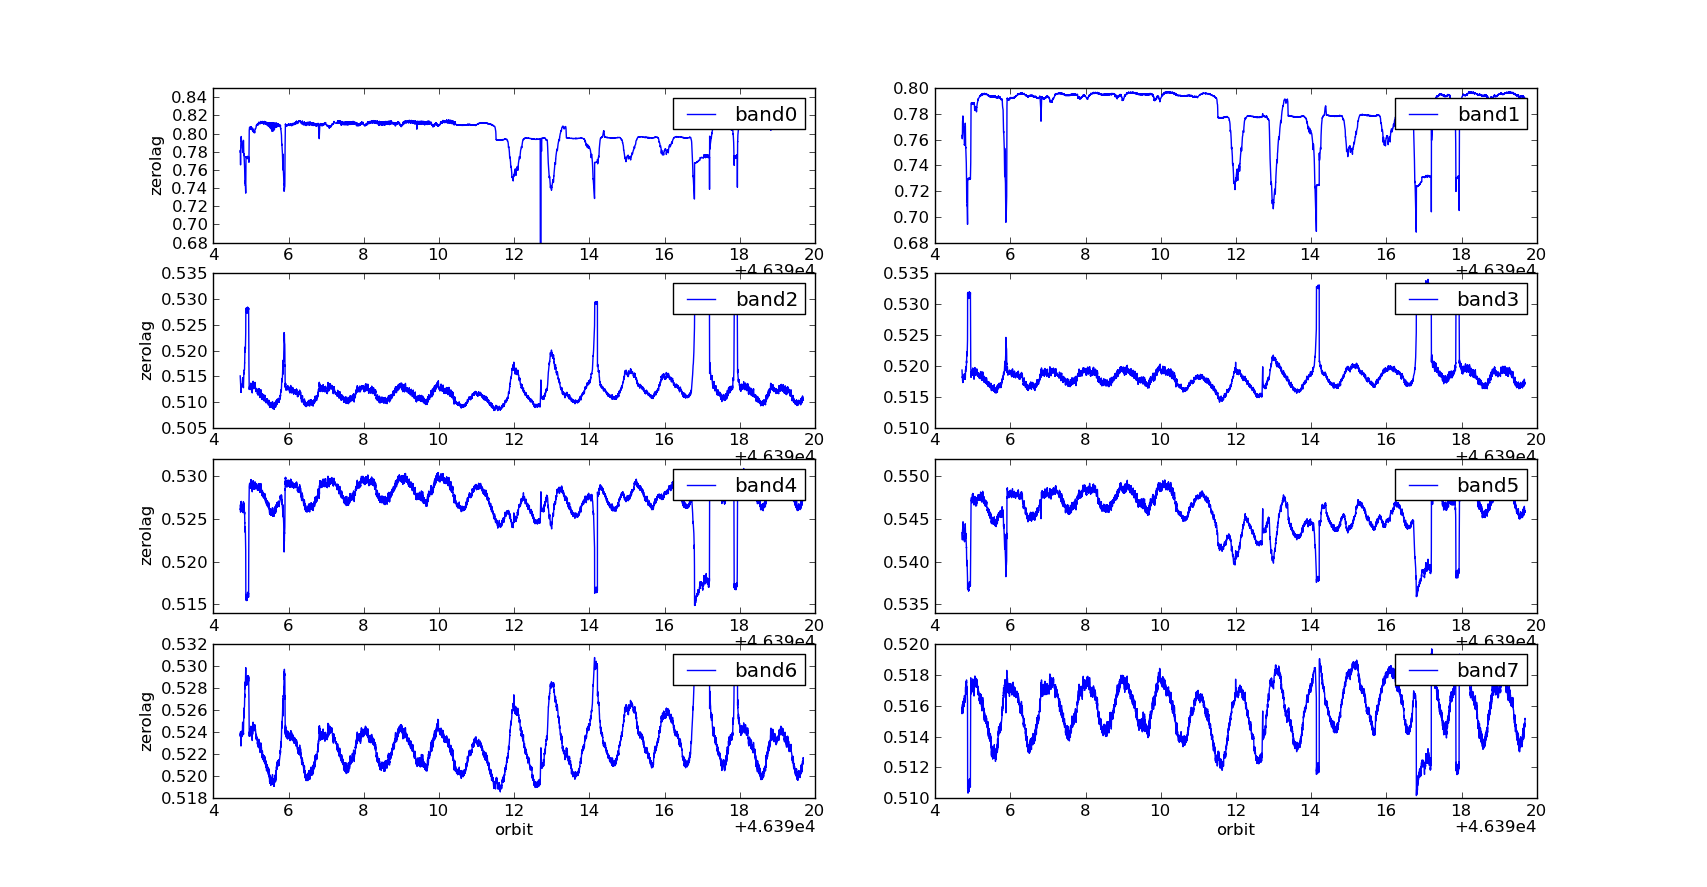
\includegraphics[scale=0.35]{ac1zerolag20orbits.png}
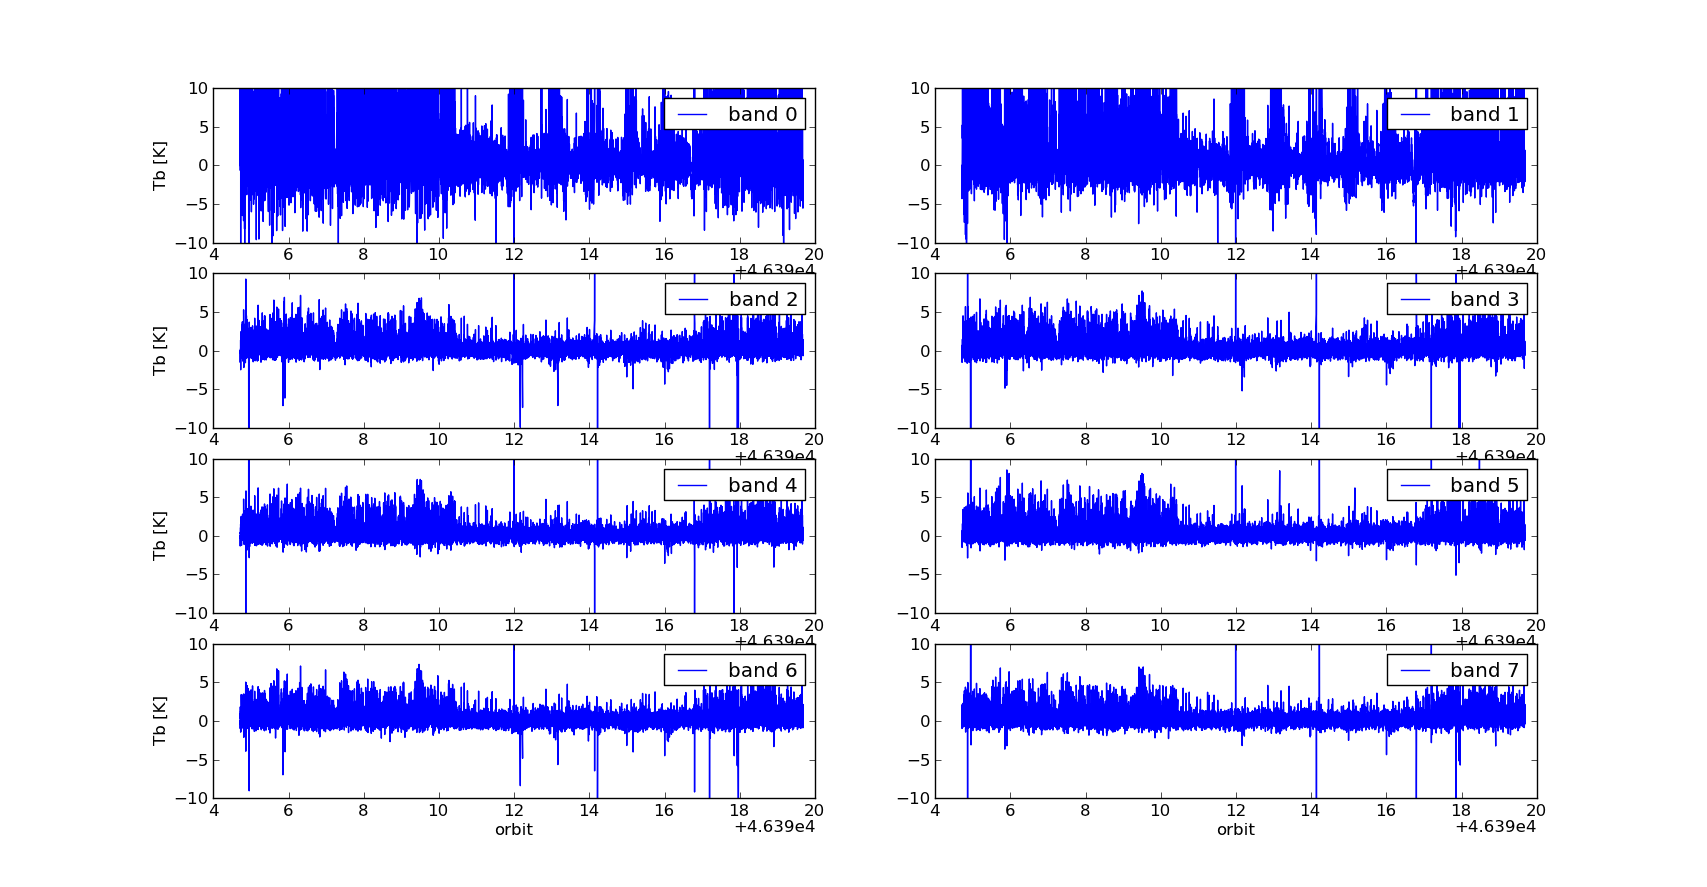
\includegraphics[scale=0.35]{ac1skysig.png}
\caption{The upper panels shows zerolags for AC1 (same as Figure~\ref{fig:study1ac1c}) and the lower panels shows the mean Tb of calibrated sky signal of each band.}
\label{fig:study1ac1skysig}
\end{figure} 


  
%%%%%%%%%%








\clearpage
\newpage

\part*{Part II \newline
Spectral features and compensation}
\addcontentsline{toc}{part}{Part II \newline Spectral features and compensation }
\fancyhead[RO,RE]{\bfseries Part II: Spectral features and compensation  }
\setcounter{section}{0}
\section{Overview}
From earlier calibration versions of data from the autocorrelators
of Odin-SMR we know that calibrated spectra from both high and 
low altitudes contain spectral features not caused by the atmospheric
species.
This short report contains a likely explanation
of how these spectral features are induced
and how they affect the spectra.


\clearpage
\newpage

\section{Spectral features in spectra}
\begin{figure}[!t]
\centering
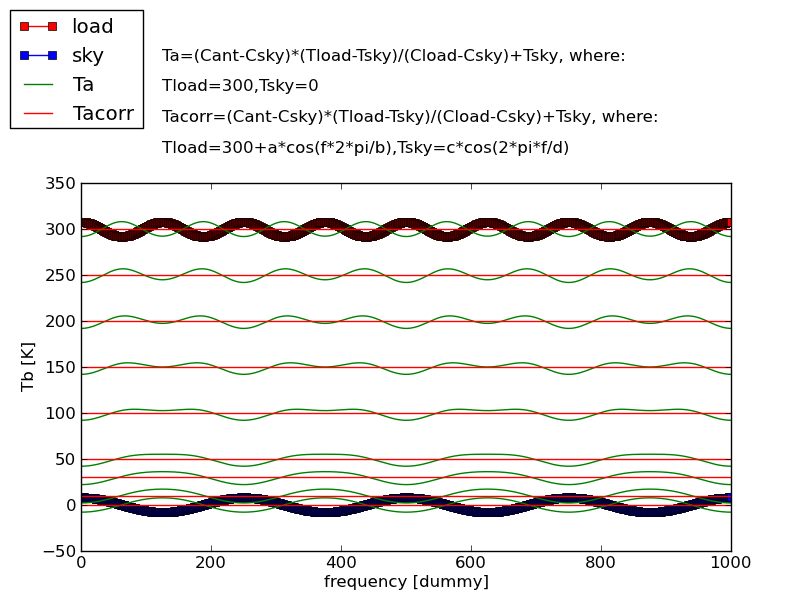
\includegraphics[scale=0.7]{odinspectrumpattern.png}\\
\caption{Wave induced pattern in calibrated spectra. The red line represents 
a perturbed brightness temperature spectrum of the
hot load (a cosinus wave with eight cycles is added)
The blue line represents a perturbed brightness temperature
spectrum of the cold sky (a cosinus wave with four cycles is added).
The thin red lines represent perfectly calibrated spectra.
The green lines show what features the cosinus waves of the
references induce on calibrated spectra if they are not taken into account.
}
\label{fig:study2ac2a}
\end{figure}

From earlier calibration versions of data from the autocorrelators
of Odin-SMR we know that calibrated spectra from both high and 
low altitudes contain spectral features not caused by the atmospheric
species. 
The spectral features, which are different at low and and high altitudes, 
are instead caused by the instrument itself and not taken into account
in the calibration process.

The calibration process (level1a to level1b) is based on that we have 
measurements of the clod sky (\(C_{s}(f)\) at 2.7 K), hot load (\(C_{L}(f)\)
at around 290 K), and the target atmosphere (\(C_{A}(f)\) 
at unkown temperature \(T_{A}\)).
The calibration process can be understand as a linear interpolation
of \(C_{A}(f)\)  using \(C_{s}(f)\) and \(C_{L}(f)\) and their temperatures
as references.
 
The calibration process assumes that both the cold sky and hot load signal
are clean. Figure~\ref{fig:study2ac2a} shows an example of what would happen with
calibrated spectra if these signals are not clean
(but the target signal is clean).
In the example the blue line represents a perturbed brightness temperature
spectrum of the cold sky (a cosinus wave with four cycles is added).
The red line represents a perturbed brightness temperature spectrum of the
hot load (a cosinus wave with eight cycles is added).
The thin red lines can be interpreted as perfectly calibrated spectra.

The green lines show what features the cosinus waves of the
references induce on calibrated spectra if they are not taken into account:

At low brightness temperatures this pattern is caused by the
the wave on the cold sky signal (and 180 degree phase shifted
w.r.t. wave on the cold sky signal).

At high brightness temperatures this pattern is caused by the
the wave on the hot load signal (and 180 degree phase shifted
w.r.t. wave on the hot load signal).

At intermediate brightness temperatures the pattern is a linear
combination of the mentioned pattern,
i.e. (using the equations in the figure) 
\begin{equation}
\Delta T=c \cdot cos\left(\frac{f2\pi}{d}+\pi\right) \cdot (1-w(f)) 
+a \cdot cos \left( \frac{f2\pi}{b}+\pi \right) \cdot w(f)
\end{equation}
where
\begin{equation}
w(f)=\frac{C_{A}(f)-C_{s}(f)}{C_{L}(f)-C_{S}(f)}\approx\frac{T_{A}(f)}{T_{L}(f)}
\end{equation}

\section{Odin data}
\subsection{AC2}
\begin{figure}[!t]
\centering
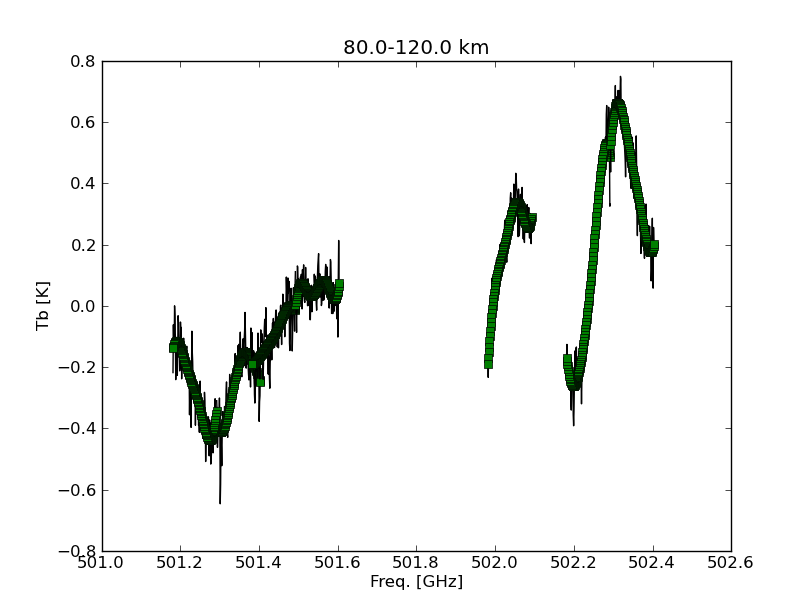
\includegraphics[scale=0.7]{ac2spechigh.png}\\
\caption{High tangent altitude median spectrum from AC2 (strat 1).}
\label{fig:study2spec1}
\end{figure}

\begin{figure}[!t]
\centering
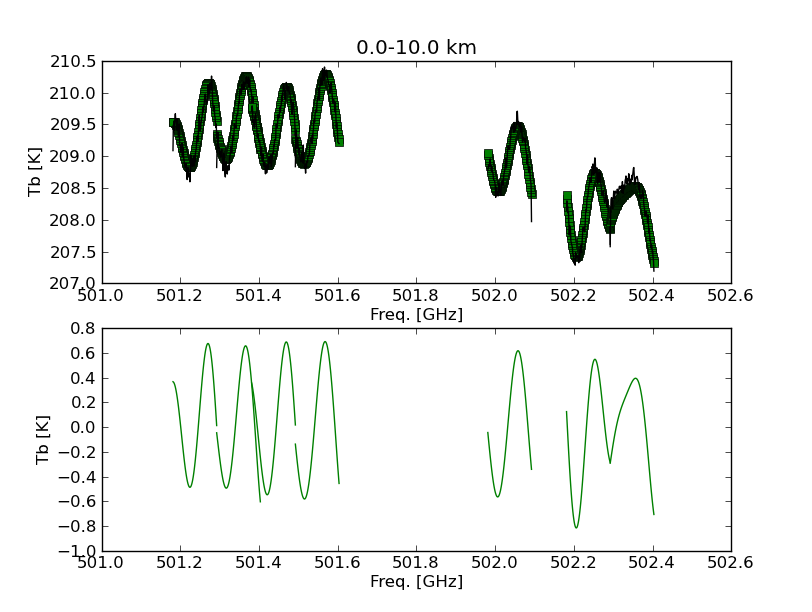
\includegraphics[scale=0.7]{ac2speclow.png}\\
\caption{Low tangent altitude median spectrum from AC2 (strat 1).}
\label{fig:study2spec2}
\end{figure}

\begin{figure}[!t]
\centering
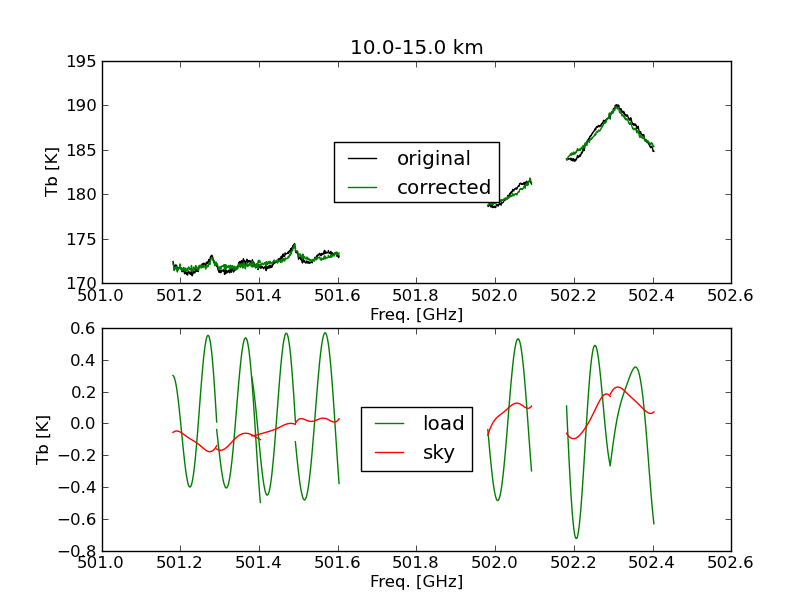
\includegraphics[scale=0.7]{ac2spec1015.png}\\
\caption{Intermediate tangent altitude median spectrum from AC2 (strat 1).}
\label{fig:study2spec3}
\end{figure}

\begin{figure}[!t]
\centering
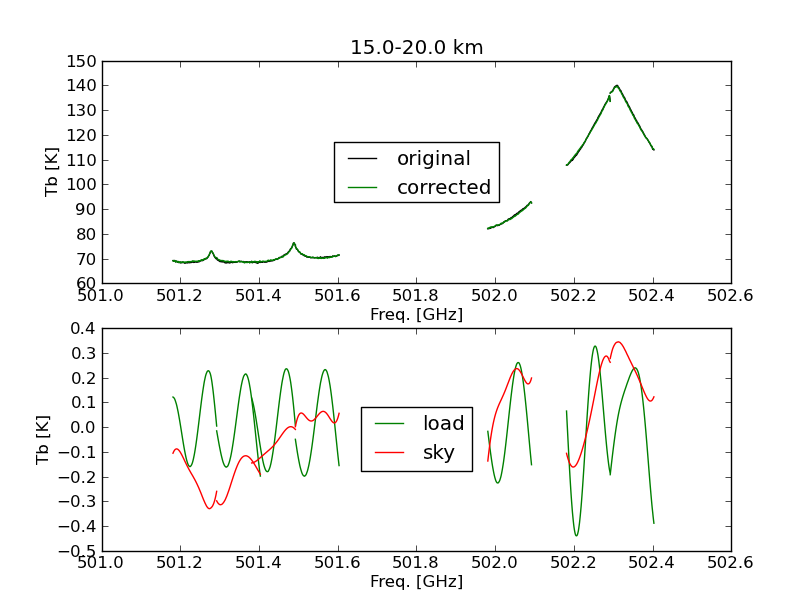
\includegraphics[scale=0.7]{ac2spec1520.png}\\
\caption{Intermediate tangent altitude median spectrum from AC2 (strat 1).}
\label{fig:study2spec4}
\end{figure}

\begin{figure}[!t]
\centering
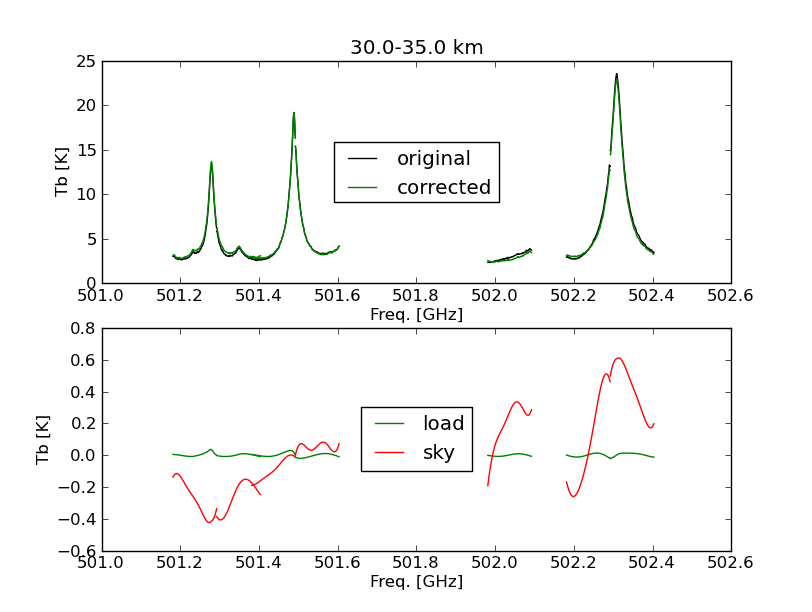
\includegraphics[scale=0.7]{ac2spec3035.png}\\
\caption{Intermediate tangent altitude median spectrum from AC2 (strat 1).}
\label{fig:study2spec5}
\end{figure}

\begin{figure}[!t]
\centering
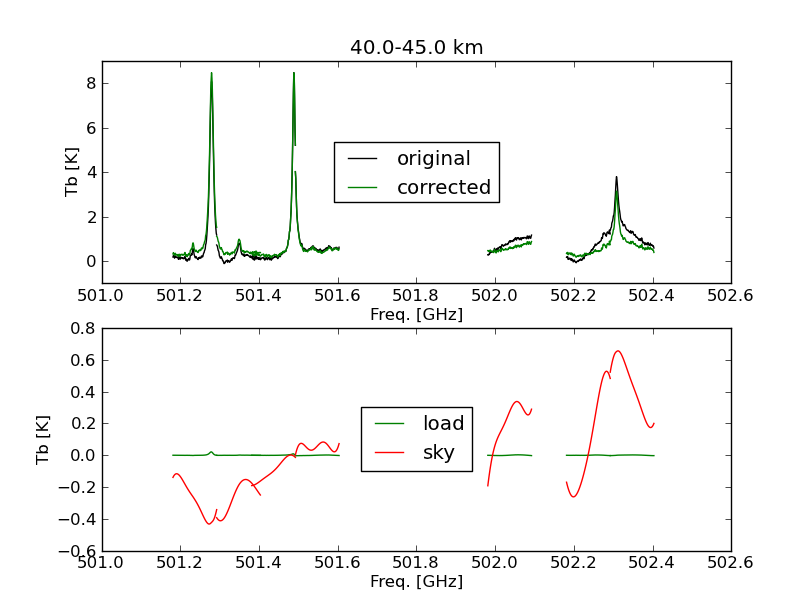
\includegraphics[scale=0.7]{ac2spec4045.png}\\
\caption{Intermediate tangent altitude median spectrum from AC2 (strat 1).}
\label{fig:study2spec6}
\end{figure}

\begin{figure}[!t]
\centering
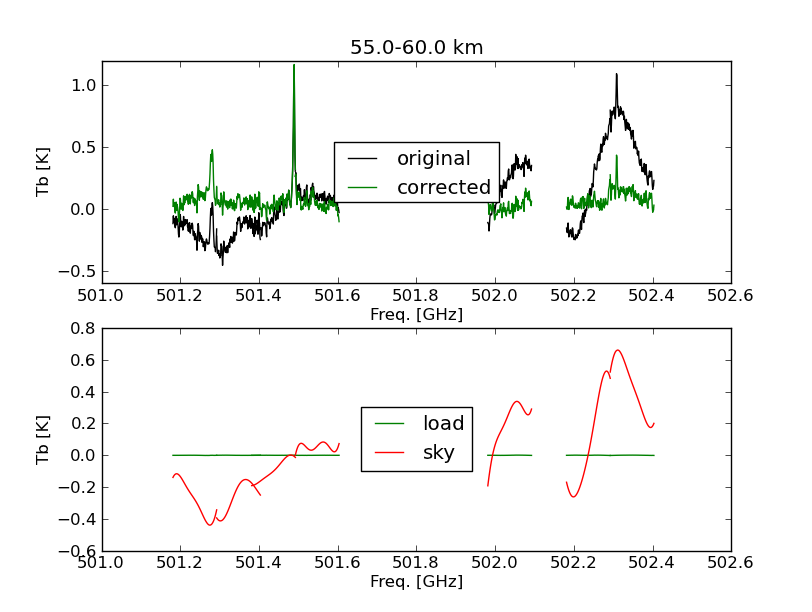
\includegraphics[scale=0.7]{ac2spec5560.png}\\
\caption{Intermediate tangent altitude median spectrum from AC2 (strat 1).}
\label{fig:study2spec7}
\end{figure}
\clearpage
\newpage
\subsection{AC1}
\begin{figure}[!t]
\centering
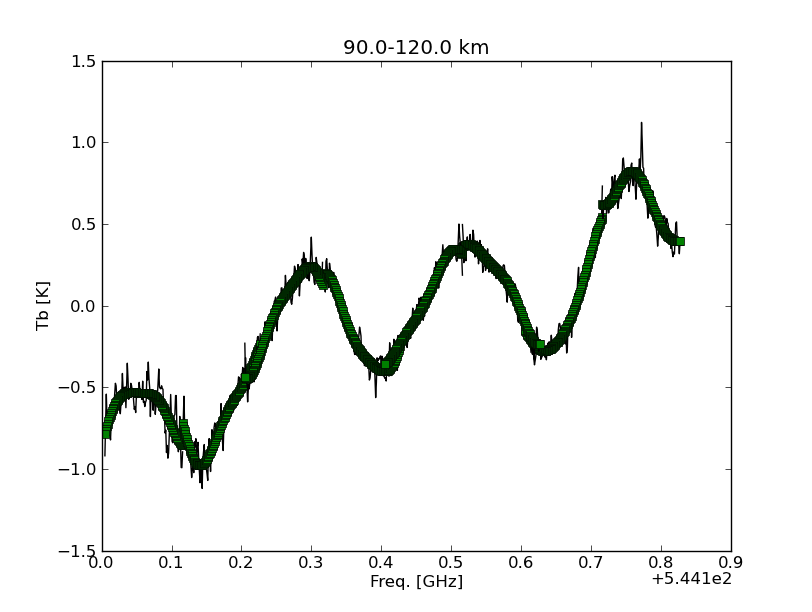
\includegraphics[scale=0.7]{ac1spechigh.png}\\
\caption{High tangent altitude median spectrum from AC1 (strat 2).}
\label{fig:study2spec8}
\end{figure}

\begin{figure}[!t]
\centering
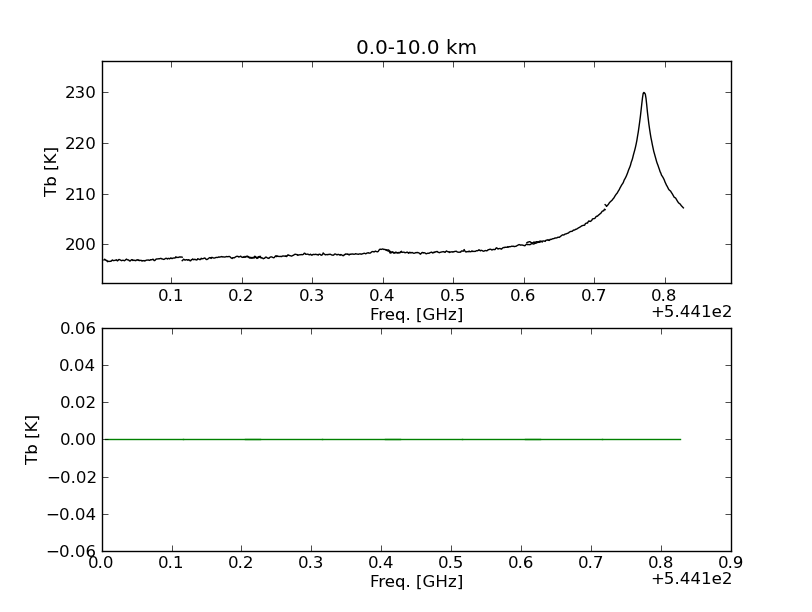
\includegraphics[scale=0.7]{ac1speclow.png}\\
\caption{Low tangent altitude median spectrum from AC1 (strat 2).}
\label{fig:study2spec9}
\end{figure}



\begin{figure}[!t]
\centering
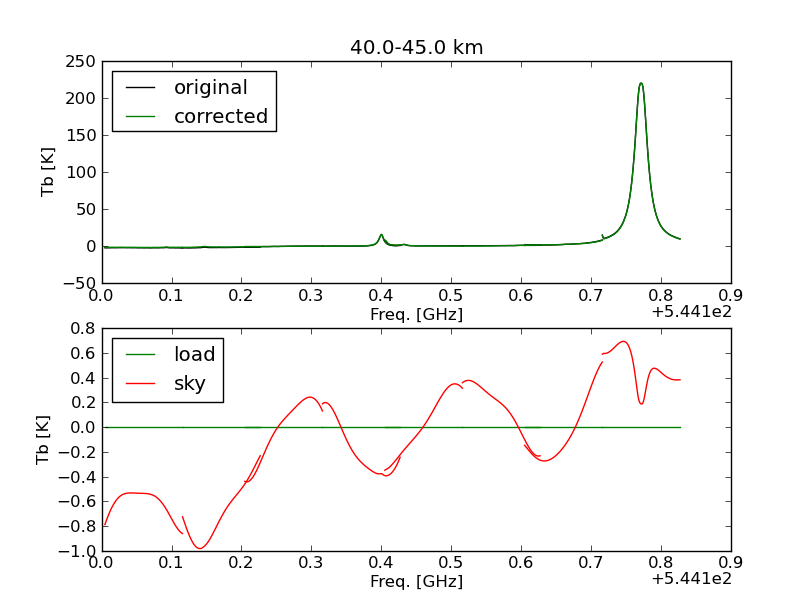
\includegraphics[scale=0.7]{ac1spec4045.png}\\
\caption{Intermediate tangent altitude median spectrum from AC1 (strat 2).}
\label{fig:spec1}
\end{figure}

\begin{figure}[!t]
\centering
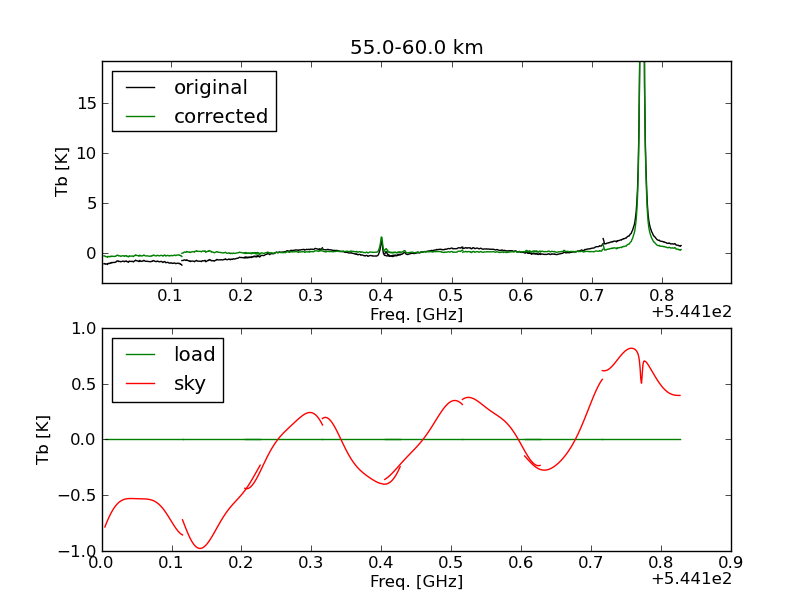
\includegraphics[scale=0.7]{ac1spec5560.png}\\
\caption{Intermediate tangent altitude median spectrum from AC1 (strat 2).}
\label{fig:spec1}
\end{figure}







\clearpage
\newpage


\part*{Part III \newline
Calibration of sky signals}
\addcontentsline{toc}{part}{Part III \newline Calibration of sky signals }
\fancyhead[RO,RE]{\bfseries Part III: Calibration of sky signals}
\setcounter{section}{0}
\section{Overview}
This report contains figures related to the calibration
process of autocorrelator data from Odin-SMR.\\
\newline
Topics examined are:\\
\newline
Calibration of sky signals\\
The statistics of calibrated sky signals seems to be fine
except that mean and median spectra deviates from 0 K
(overestimation of sky signal with up to\(\sim\)0.3 K).
The reason for this should most likely be due to that
the gain varies (for some reason) in a systematic non-linear manner
in such a way that linear interpolation
of reference signals give rise to a systematic error
in the calibration procedure.\\
\newline
Spectral feature in high altitude spectrum\\
The spectral features seen in high altitude spectra are
examined. Spectra are sorted in temperature bins
using hotload temperature as a reference.
It is shown that the phase of the signal seen in high
altitude spectra varies with temperature.
%Thus it seems possible to remove this spectral
%feature from spectra in the calibration procedure by something like:\\
%*first perform the ``standard'' calibration
%*create a table with results from high 
%altitude measurements and e.g. hotload temperatures
%*Perform a second calibration
%\\
\clearpage
\newpage

\section{Calibration of sky signals}
In this section results from the calibration of sky signals
from AC2 (stratospheric mode 1) and AC1 (stratospheric mode 2)
are shown. The shape and statistics of calibrated skysignal
spectra from several orbits are explored.  

The calibration of sky signals is done by:
\begin{equation}
\label{eq:skysig}
T^{'}_{sky}=\frac{c_{sky}-c^{'}_{sky}}{g^{'}}+T_{sky}\approx(\frac{g}{g^{'}}-1)T_{sys},
\end{equation}
where \(T^{'}_{sky}\) is the estimation of the brightness temperature
of the sky signal, \(c_{sky}\approx g(T_{sys}+T_{sky})\approx gT_{sys}\) is the measured sky signal,
 \(c^{'}_{sky}\) is the reference estimated sky signal
which is retrieved using linear interpolation w.r.t. time using
the measured skysignals around the target \(c_{sky}\),   
\(g\) is the true
gain, and \(g^{'}\) is the estimated gain, \(T_{sys}\) is the system
noise temperature. 

Equation~\ref{eq:skysig} gives that, even if the gain varies
linearly with time and that we can estimate \(g^{'}=g+\Delta g\) with
an error \(\Delta g\) that is gaussian distributed and has zero mean,
we would expect the average sky signal spectrum to deviate from 
0 K. The simple reason for this is that a positive and negative
error in gain will not totally cancel out, i.e. 
\(\frac{g}{g+\Delta g} \neq \frac{g}{g-\Delta g}\).    
However, in this case the median spectrum would be very close to
0 K.
In this section it is shown that both mean and median of calibrated
skysignal spectra deviates from 0 K.


\clearpage
\newpage

\subsection{AC2}
\begin{figure}[!t]
\centering
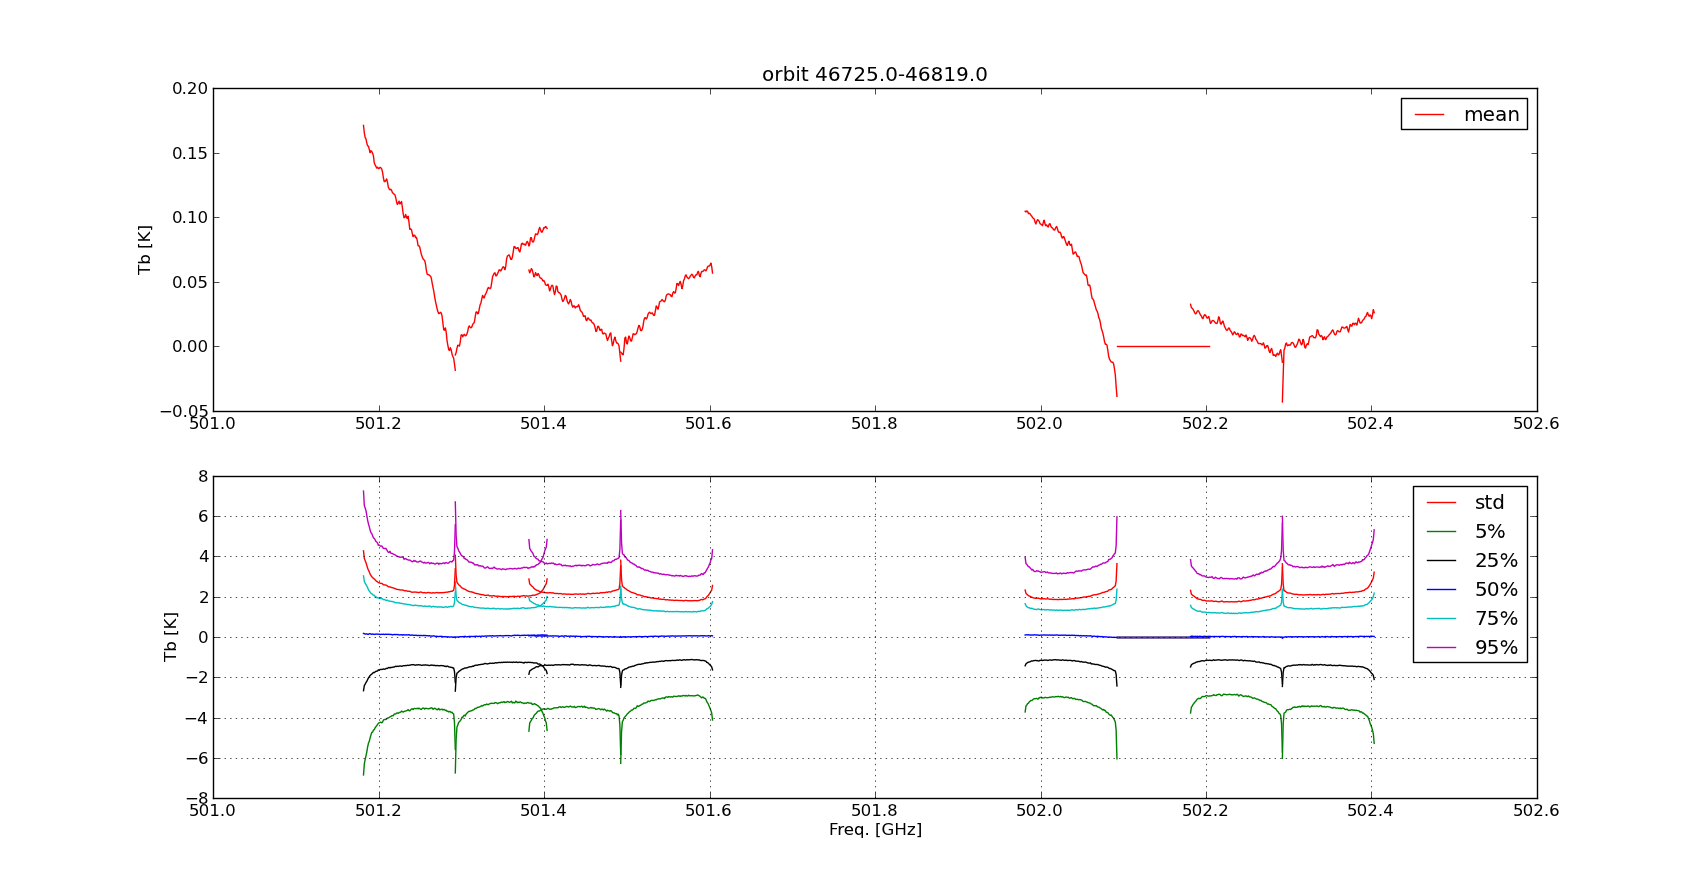
\includegraphics[scale=0.35]{ac2skycal1.png}\\
\caption{The upper panel shows a mean spectrum of calibrated
skysignals from AC2 stratospheric mode 1. 
The lower panel show a standard deviation spectrum
and percentiles spectra.}
\label{fig:study3ac2a}
\end{figure}

\begin{figure}[!t]
\centering
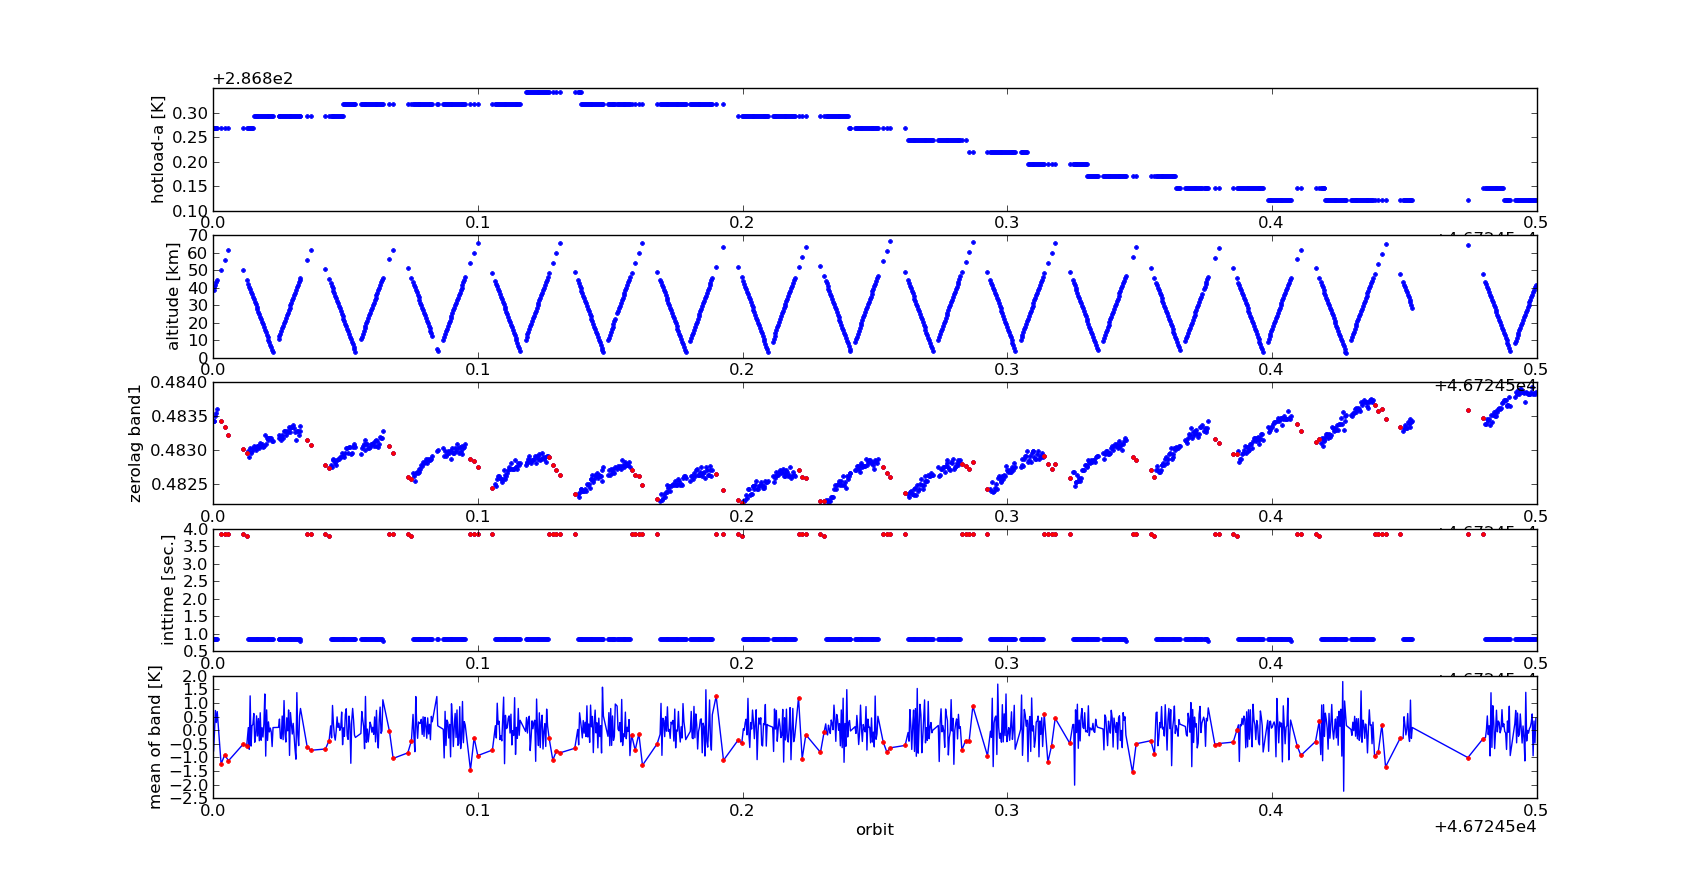
\includegraphics[scale=0.35]{ac2skycal2.png}\\
\caption{Time series of various data from part of an orbit.
The upper (first) panel shows hotload temperatures.
The second panel shows tangent altitudes.
The third panel shows zerolags of skysignals for band 1 of AC2.
The fourth panel shows integration times.
The lower panel shows band 1 average calibrated brightness temperatues.}
\label{fig:study3ac2b}
\end{figure}


The upper panel of Figure~\ref{fig:study3ac2a} shows a mean spectrum
of calibrated sky signals from several orbits. It can clearly be seen
that this spectrum deviates from 0 K (approximately the true brightness 
temperature of the sky signal).
The lower panel shows some additional statistics.
The standard deviation of the spectrum is around 2 K,
which agrees well with the expected theoretical noise level
(\(\Delta T =T_{sys}/\sqrt{B*\tau} \approx 3000 K / \sqrt{2MHz*1s}=2.1 K\)).
The percentiles (for example the 25 and 75) are fairly evenly
displaced from the 50\% percentile (median),
which means that the errors are at least close to gaussian
distributed.  
The median has the same pattern as the mean (which is hard to see
due to the scale).

The reason for the median deviation from 0 K is most likely due to 
some systematic gain variations, i.e. the gain does not vary
completely linearly with time between three sky signals
measurements.

%Equation~\ref{eq:skysig} gives that, even if the gain varies
%linearly with time and that we can estimate \(g^{'}=g+\Delta g\) with
%an error \(\Delta g\) that is gaussian distributed and has zero mean,
%we would expect the average sky signal spectrum to deviate from 
%zero. The simple reason for this is that a positive and negative
%error in gain will not totally cancel out, i.e. 
%\(\frac{g}{g+\Delta g} \neq \frac{g}{g-\Delta g}\).
%However, since \(\Delta g\) in general is very small this
%does not explain the shape of the median spectrum in Figure~\ref{fig:ac2a}. 

Figure~\ref{fig:study3ac2b} show time series of various data from 
part of an orbit.
The middle panel shows the variation of zerolags for band 1
of AC2 (the variation of zerolags from other bands looks similiar).
On a short time scale (over one scan down and up) the zerolags increases
until the 4 seconds integration time starts. Then zerolags decreases
during the period with four seconds integration times. 
It seems that for the time period when zerolags increases
the increase is not totally linear in time.

This means that on average we probably make a systematic
error or underestimation of \(c^{'}_{sky}\) in the calibration
procedure, which means that we overestimate \(T^{'}_{sky}\)
(see Equation~\ref{eq:skysig}).
To overcome this problem a possible solution would be to use a weighted
quadratic interpolation as we have earlier discussed.

\clearpage
\newpage
\subsection{AC1}

\begin{figure}[!t]
\centering
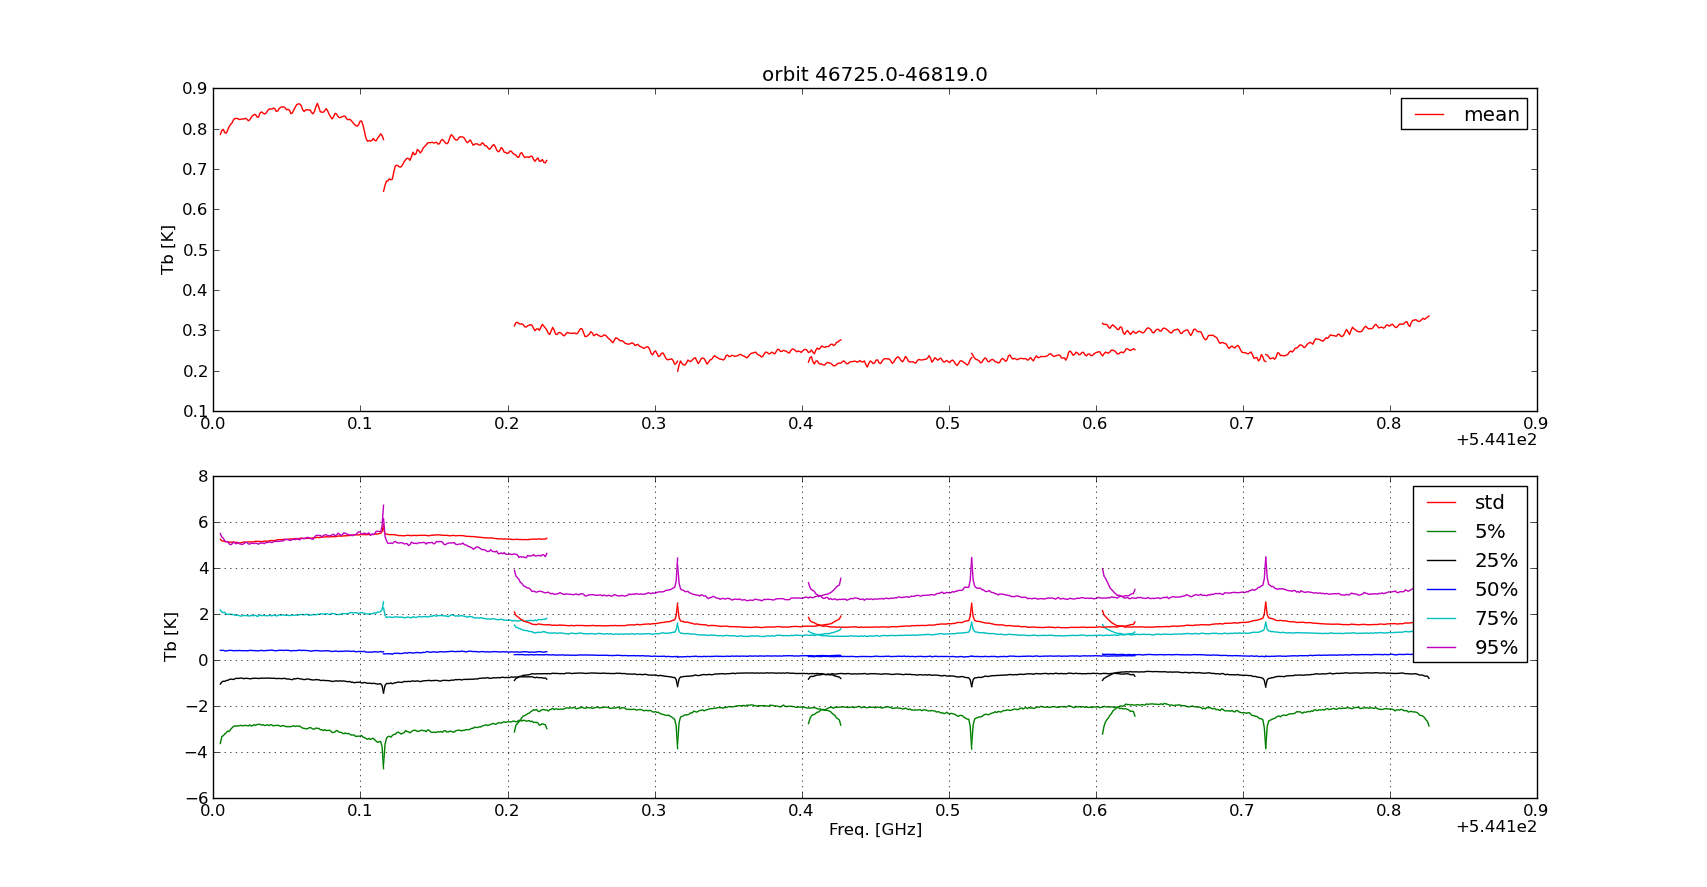
\includegraphics[scale=0.35]{ac1skycal1.png}\\
\caption{The upper panel shows a mean spectrum of calibrated
skysignals from AC1 stratospheric mode 2. 
The lower panel show a standard deviation spectrum
and percentiles spectra.}
\label{fig:study3ac1a}
\end{figure}

\begin{figure}[!t]
\centering
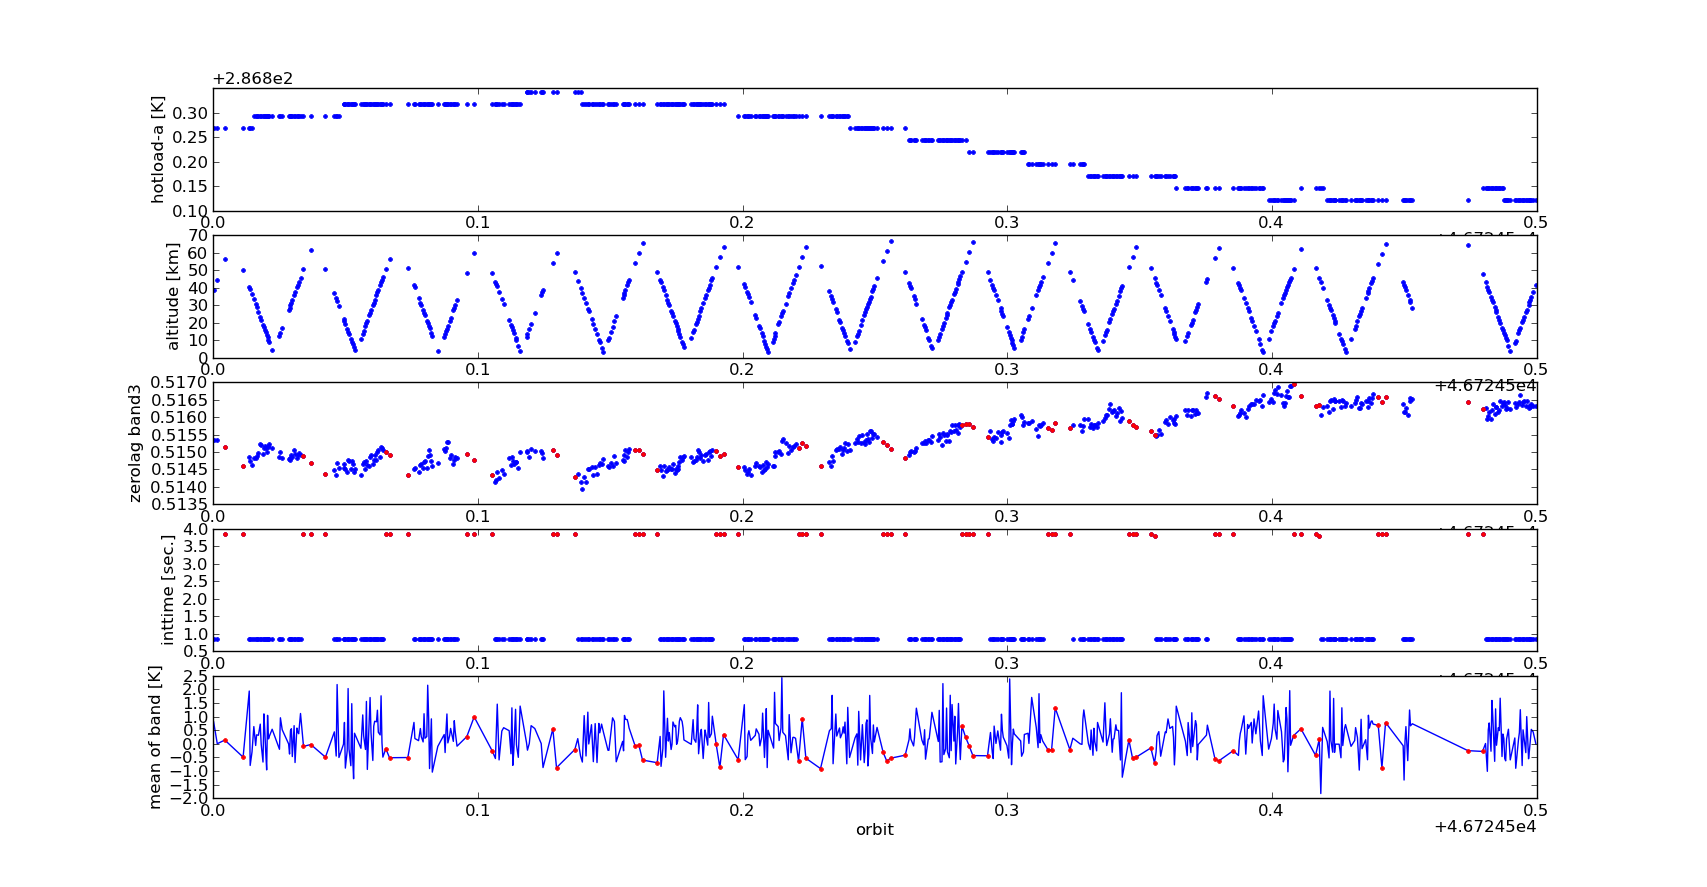
\includegraphics[scale=0.35]{ac1skycal2.png}\\
\caption{Time series of various data from part of an orbit.
The upper (first) panel shows hotload temperatures.
The second panel shows tangent altitudes.
The third panel shows zerolags of skysignals for band 3 of AC1.
The fourth panel shows integration times.
The lower panel shows band 1 average calibrated brightness temperatues.}
\label{fig:study3ac1b}
\end{figure}

 
Figures~\ref{fig:study3ac1a} and~\ref{fig:study3ac1b} show corresponding
data as Figures~\ref{fig:study3ac2a} and~\ref{fig:study3ac2b}
but for AC1 (stratospheric mode 2).
The results look very similiar for AC1 as for AC2.
The statistics of calibrated sky signals looks as expected
except that mean and median values deviates from 0 K
with around 0.25 K (Figure~\ref{fig:study3ac1a}),
except the two problematic bands in the lower part of the
spectrum.
Similiar pattern of short time scale variations in zerolag
as for AC2 is obsereved (Figure~\ref{fig:study3ac1b}).


\clearpage
\newpage
\section{High altitude spectra}   
\begin{figure}[!t]
\centering
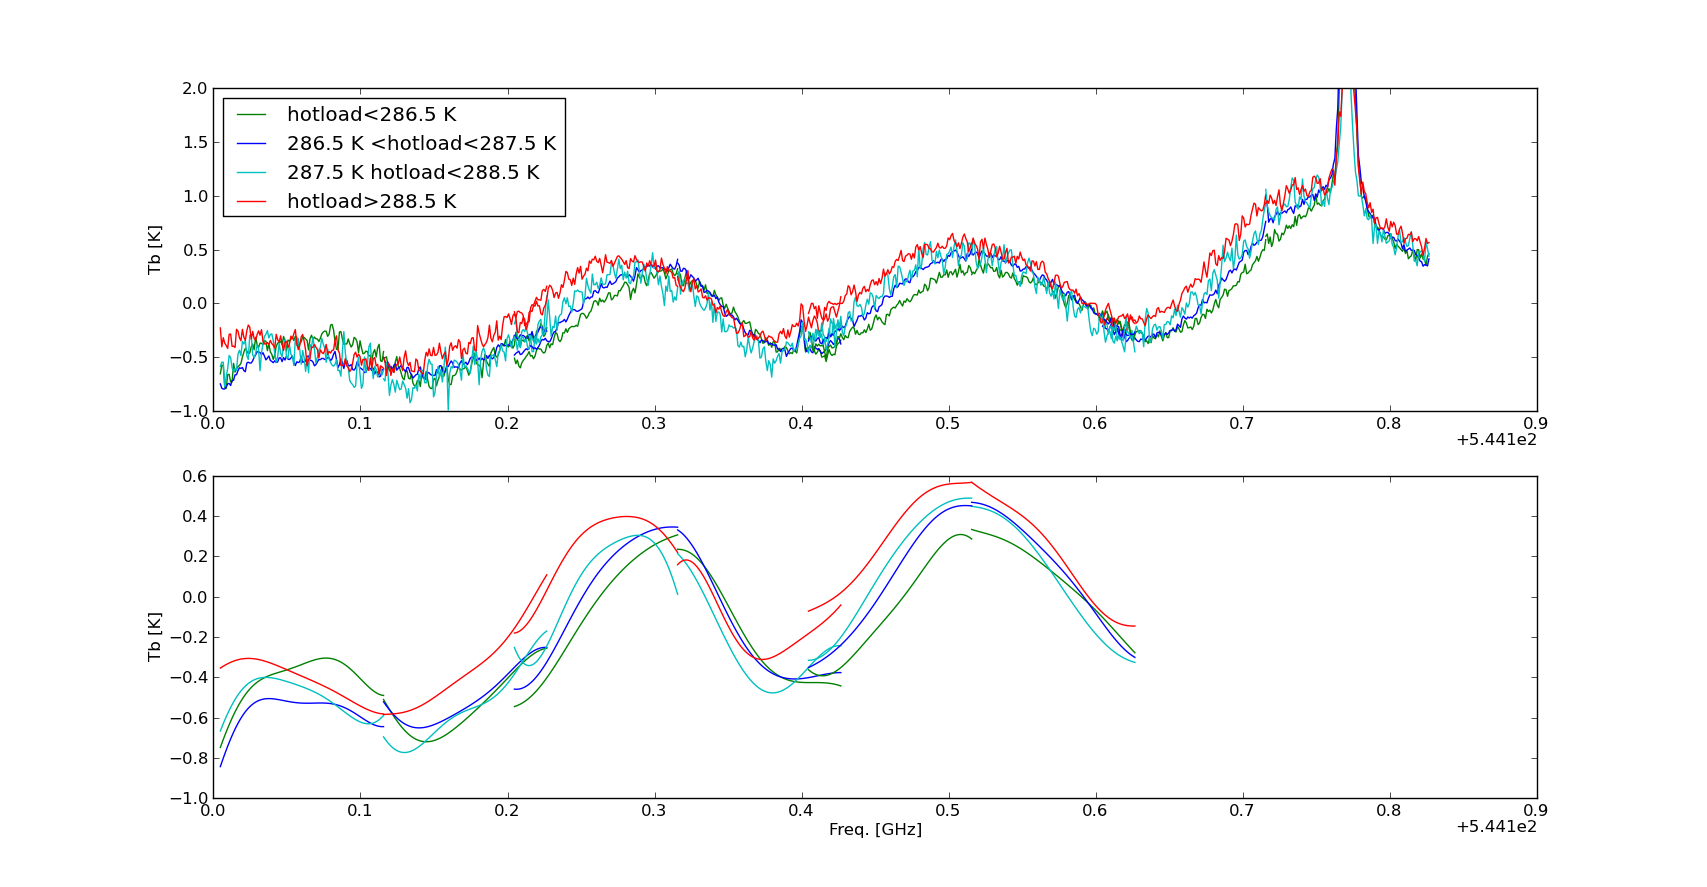
\includegraphics[scale=0.35]{ac1highalt.png}\\
\caption{The upper panel show median of high altitude (60-120 km)
spectra for different temperatures for AC1 stratospheric mode 2.
The lower panel shows fits to spectra in the upper panel.}
\label{fig:study3ac1c}
\end{figure}

\begin{figure}[!t]
\centering
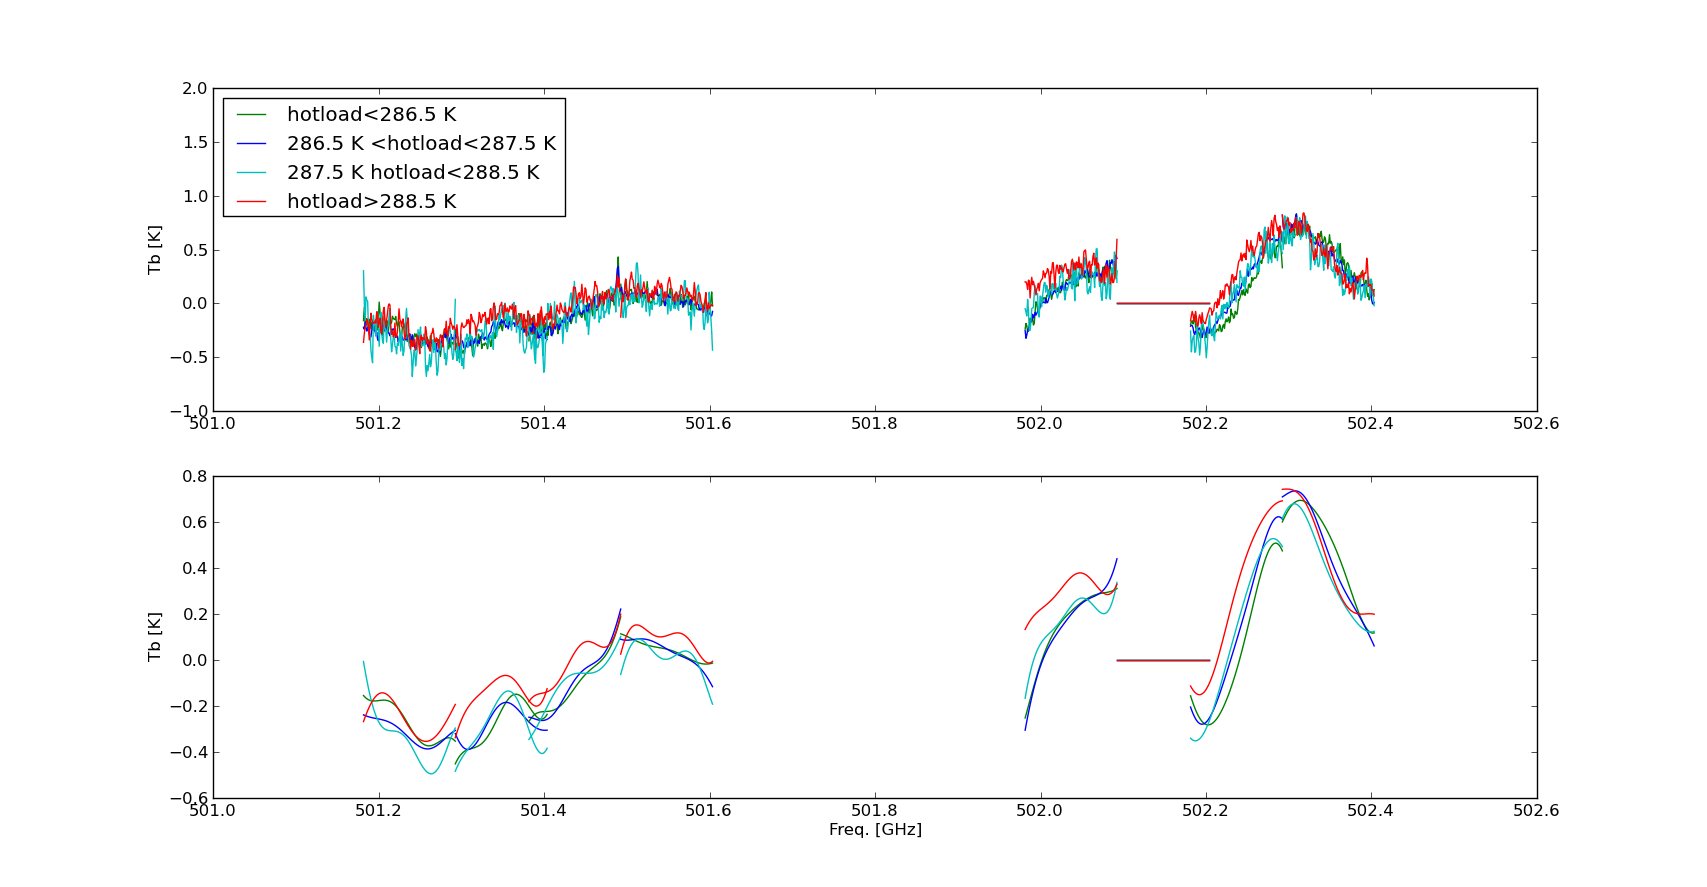
\includegraphics[scale=0.35]{ac2highalt.png}\\
\caption{The upper panel show median of high altitude (60-120 km)
spectra for different temperatures for AC2 stratospheric mode 1.
The lower panel shows fits to spectra in the upper panel.}
\label{fig:study3ac2c}
\end{figure}


In this section high altitude spectra from AC1 and AC2 are explored.
We know from earlier studies that these spectra contains
spectral features even though we do not expect this.
This spectral features should come from that either the sky signal
or the target signal is perturbed. Most likely it comes from ripple on the
sky signal. Regardless where it comes from, it should be possible to remove
this spectral feature in the calibration process. Although, the way to
properly remove it depends on where it comes from.

However, in this section we look at the temperature dependence
of the spectral features. Figures~\ref{fig:study3ac1c} and~\ref{fig:study3ac2c}
shows median of calibrated high altitude measurements from around 
200 orbits from 2009-08-24 to 2009-09-24. 
The data is sorted in temperature bins using the hotload temperature
as reference temperature.   
Figure~\ref{fig:study3ac1c} shows that the phase of the signal seen in AC1 
high altitude measurements varies with temperature.
This effect can also be seen in Figure~\ref{fig:study3ac2c} for AC2
although it is not so clear as for AC1.









\clearpage
\newpage

\part*{Part IV \newline
Reference interpolation }
\addcontentsline{toc}{part}{Part IV \newline Reference interpolation }
\fancyhead[RO,RE]{\bfseries Part IV: Reference interpolation}
\setcounter{section}{0}
\section{Overview}
This report contains figures related to the calibration
process of autocorrelator data from Odin-SMR.\\
\newline
The topic examined is:\\
\newline
Calibration of sky signals using linear and quadratic interpolations\\
The calibration of sky signals using two different interpolation
methods are compared.
The results from the two methods are very comparable
(depending a bit on the settings for the quadratic interpolation),
with statistically similar mean and median values
and similar distribution.


\clearpage
\newpage

\section{Calibration of sky signals}
We know from earlier studies that mean values
of calibrated sky signals differs somewhat from 
the expected \(T_{sky}\sim0 K\). In this report we examine
if a weighted quadratic interpolation routine
will improve the results.   



\subsection{Basics}
The calibration of sky signals is done by:
\begin{equation}
\label{eq:skysig}
T^{'}_{sky}=\frac{c_{sky}-c^{'}_{sky}}{g^{'}}+T_{sky}\approx(\frac{g}{g^{'}}-1)T_{sys},
\end{equation}
where \(T^{'}_{sky}\) is the estimation of the brightness temperature
of the sky signal, \(c_{sky}\approx g(T_{sys}+T_{sky})\approx gT_{sys}\) is the measured sky signal,
 \(c^{'}_{sky}\) is the reference estimated sky signal
which is retrieved using linear/quadratic interpolation using
the measured sky signals around the target \(c_{sky}\),   
\(g\) is the true
gain, and \(g^{'}\) is the estimated gain, \(T_{sys}\) is the system
noise temperature.
\subsection{Reference interpolation}
For each channel (\(c_{i}\)) of the autocorrelators 
we fit a second degree polynomial,
\begin{equation}
c_{i}(t)=a+bt+ct^{2},
\end{equation}
to the time series of reference measurements (\(c_{i}(t_{0})\),\(c_{i}(t_{1})\),...,\(c_{i}(t_{n})\)). For time zero a weighted quadratic fit can 
be estimated as
\begin{equation}
c_{i}(0)=\frac{1}{\Delta}\left|
\begin{array}{ccc}
\sum \frac{c_{i}(t_{j})w^{2}(t_{j})}{\sigma^{2}(t_{j})} & 
\sum \frac{t_{j}c_{i}(t_{j})w^{2}(t_{j})}{\sigma^{2}(t_{j})} &
\sum \frac{t_{j}^{2}c_{i}(t_{j})w^{2}(t_{j})}{\sigma^{2}(t_{j})}\\
\sum \frac{t_{j}c_{i}(t_{j})w^{2}(t_{j})}{\sigma^{2}(t_{j})} & 
\sum \frac{t_{j}^{2}c_{i}(t_{j})w^{2}(t_{j})}{\sigma^{2}(t_{j})} &
\sum \frac{t_{j}^{3}c_{i}(t_{j})w^{2}(t_{j})}{\sigma^{2}(t_{j})}\\
\sum \frac{t_{j}^{2}c_{i}(t_{j})w^{2}(t_{j})}{\sigma^{2}(t_{j})} & 
\sum \frac{t_{j}^{3}c_{i}(t_{j})w^{2}(t_{j})}{\sigma^{2}(t_{j})} &
\sum \frac{t_{j}^{4}c_{i}(t_{j})w^{2}(t_{j})}{\sigma^{2}(t_{j})}\\
\end{array}
\right|,
\end{equation}

\begin{equation}
\Delta=\left|
\begin{array}{ccc}
\sum \frac{w^{2}(t_{j})}{\sigma^{2}(t_{j})} & 
\sum \frac{t_{j}w^{2}(t_{j})}{\sigma^{2}(t_{j})} &
\sum \frac{t_{j}^{2}w^{2}(t_{j})}{\sigma^{2}(t_{j})}\\
\sum \frac{t_{j}w^{2}(t_{j})}{\sigma^{2}(t_{j})} & 
\sum \frac{t_{j}^{2}w^{2}(t_{j})}{\sigma^{2}(t_{j})} &
\sum \frac{t_{j}^{3}w^{2}(t_{j})}{\sigma^{2}(t_{j})}\\
\sum \frac{t_{j}^{2}w^{2}(t_{j})}{\sigma^{2}(t_{j})} & 
\sum \frac{t_{j}^{3}w^{2}(t_{j})}{\sigma^{2}(t_{j})} &
\sum \frac{t_{j}^{4}w^{2}(t_{j})}{\sigma^{2}(t_{j})}\\
\end{array}
\right|,
\end{equation}
and we use an exponential drop off weighting
\begin{equation}
w(t_{j})=exp\left(-\frac{|t_{j}|}{\lambda} \right),
\end{equation}
where \(\lambda\) controls the weighting,
and \(\sigma(t_{j})\) represents the uncertainty of each measurement
\begin{equation}
\sigma(t_{j})\sim\frac{1}{\sqrt{t_{int}}},
\end{equation}
where \(t_{int}\) is the integration time.

\subsection{Test results}

In this section we compare calibration of sky signals
using linear interpolation and the previously described
quadratic interpolation. Data from six orbits, including around
10000 sky signals, are considered. 


\subsubsection{Linear interpolation}
\begin{figure}[!t]
\centering
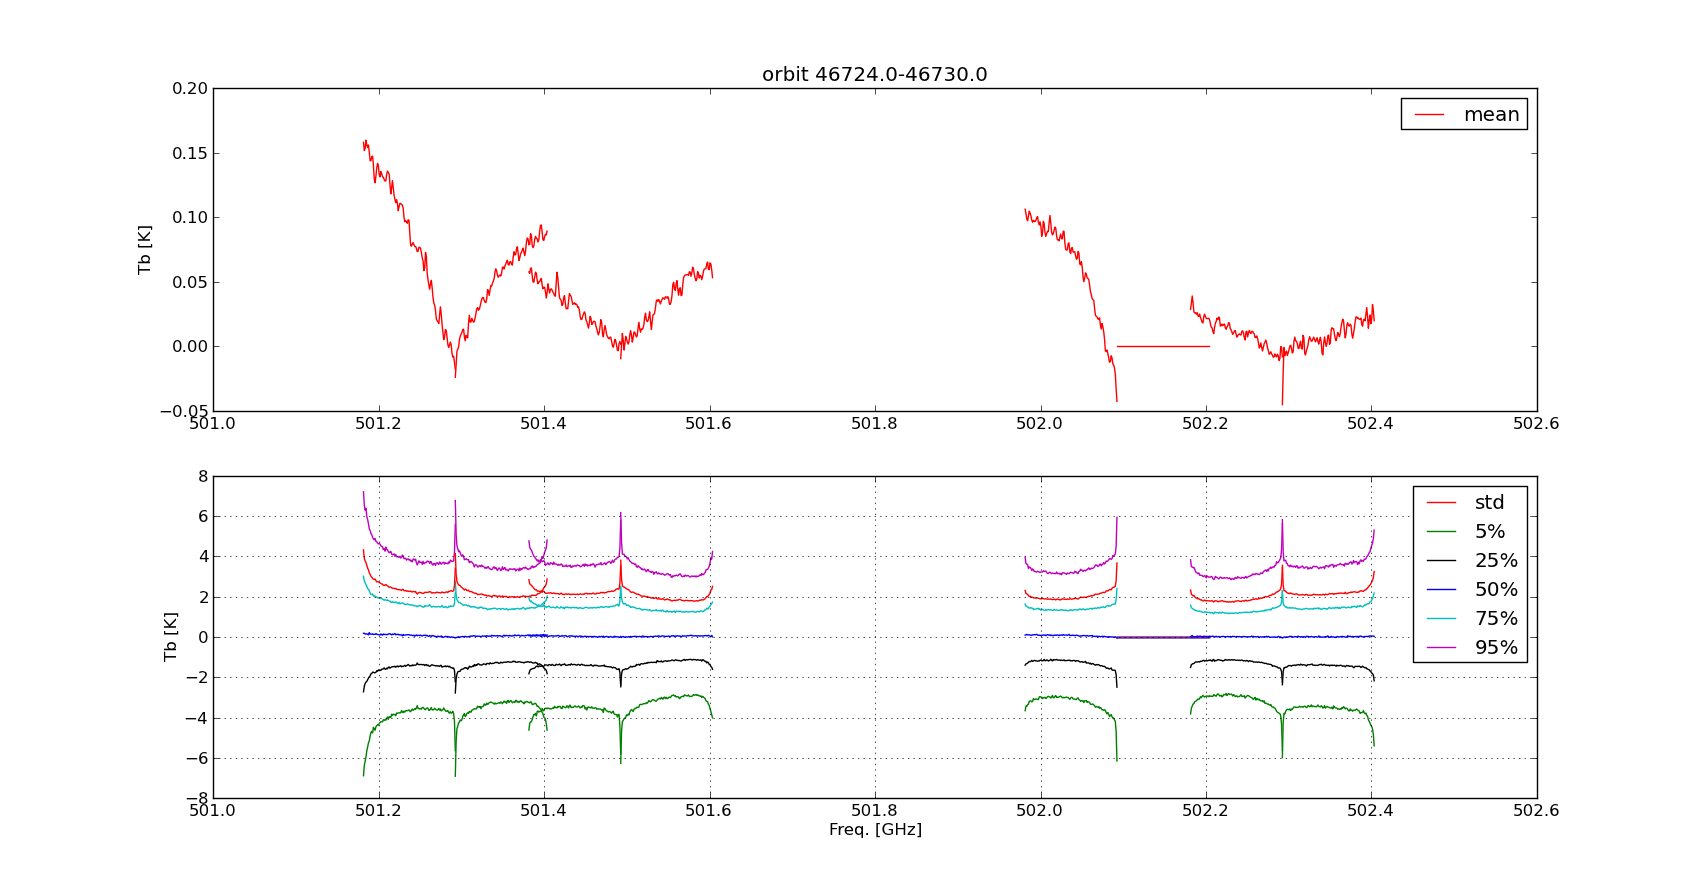
\includegraphics[scale=0.35]{study4linear.png}\\
\caption{The upper panel shows a mean spectrum of calibrated
sky signals from AC2 stratospheric mode 1,
using linear interpolation. 
The lower panel show a standard deviation spectrum
and percentiles spectra.}
\label{fig:study4linear.png}
\end{figure}

The upper panel of Figure 1 shows a mean spectrum
of calibrated sky signals from 6 orbits (~10000 sky signals). 
It can clearly be seen
that this spectrum deviates from 0 K (approximately the true brightness 
temperature of the sky signal).

The lower panel shows some additional statistics.
The standard deviation of the spectrum is around 2 K,
which agrees well with the expected theoretical noise level
(\(\Delta T =T_{sys}/\sqrt{B*\tau} \approx 3000 K / \sqrt{2MHz*0.8s}=2.37 K\)).
The percentiles (for example the 25 and 75) are fairly evenly
displaced from the 50\% percentile (median),
which means that the errors are at least close to Gaussian
distributed.  
The median has the same pattern as the mean (which is hard to see
due to the scale).

The reason for the median deviation from 0 K is most likely due to 
that the gain does not vary
completely linearly with time between three sky signals
measurements.

\subsubsection{Quadratic interpolation setup}
\begin{figure}[!t]
\centering
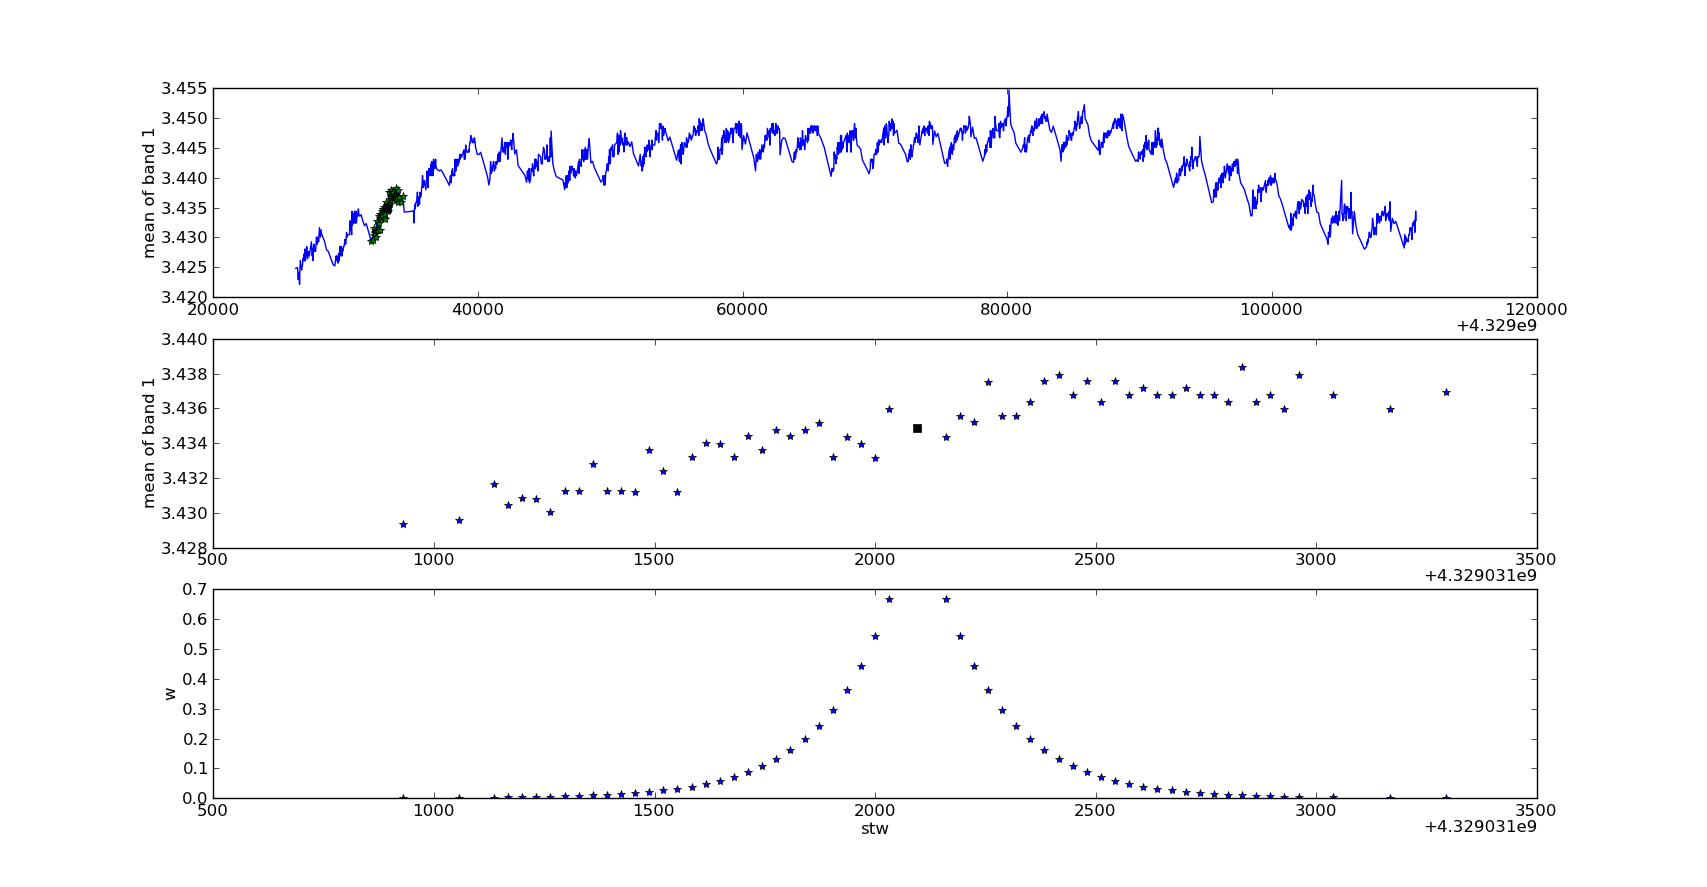
\includegraphics[scale=0.35]{study4_dem.png}\\
\caption{The upper panel shows mean of band1 of level1a data
from several scans.
The middle panel shows a zoom in of the black dots in the upper panel,
and the black square is the fitted value
(the fit is performed for each channel).
The lower panel shows the corresponding weights (x=8) of each measurement 
in the fit. }
\label{fig:study4_dem.png}
\end{figure}

The quadratic fit of a reference measurement at time \(t\)
is done in the following way (see Figure 2).  
We first find out the time-interval \(\Delta T\) of the scan that
the measurement belongs to. 
In the fit, we then consider all reference measurements
that where performed during the time interval 
\(t-\Delta T\) to \(t+\Delta T\). 
The weighting parameter \(\lambda\) is then given
the value  \(\Delta T /x\), where we tested the performance
of several values of x (4,8,16,32,64,and 128).

\clearpage
\newpage
\subsubsection{Quadratic interpolation}
\begin{figure}[!t]
\centering
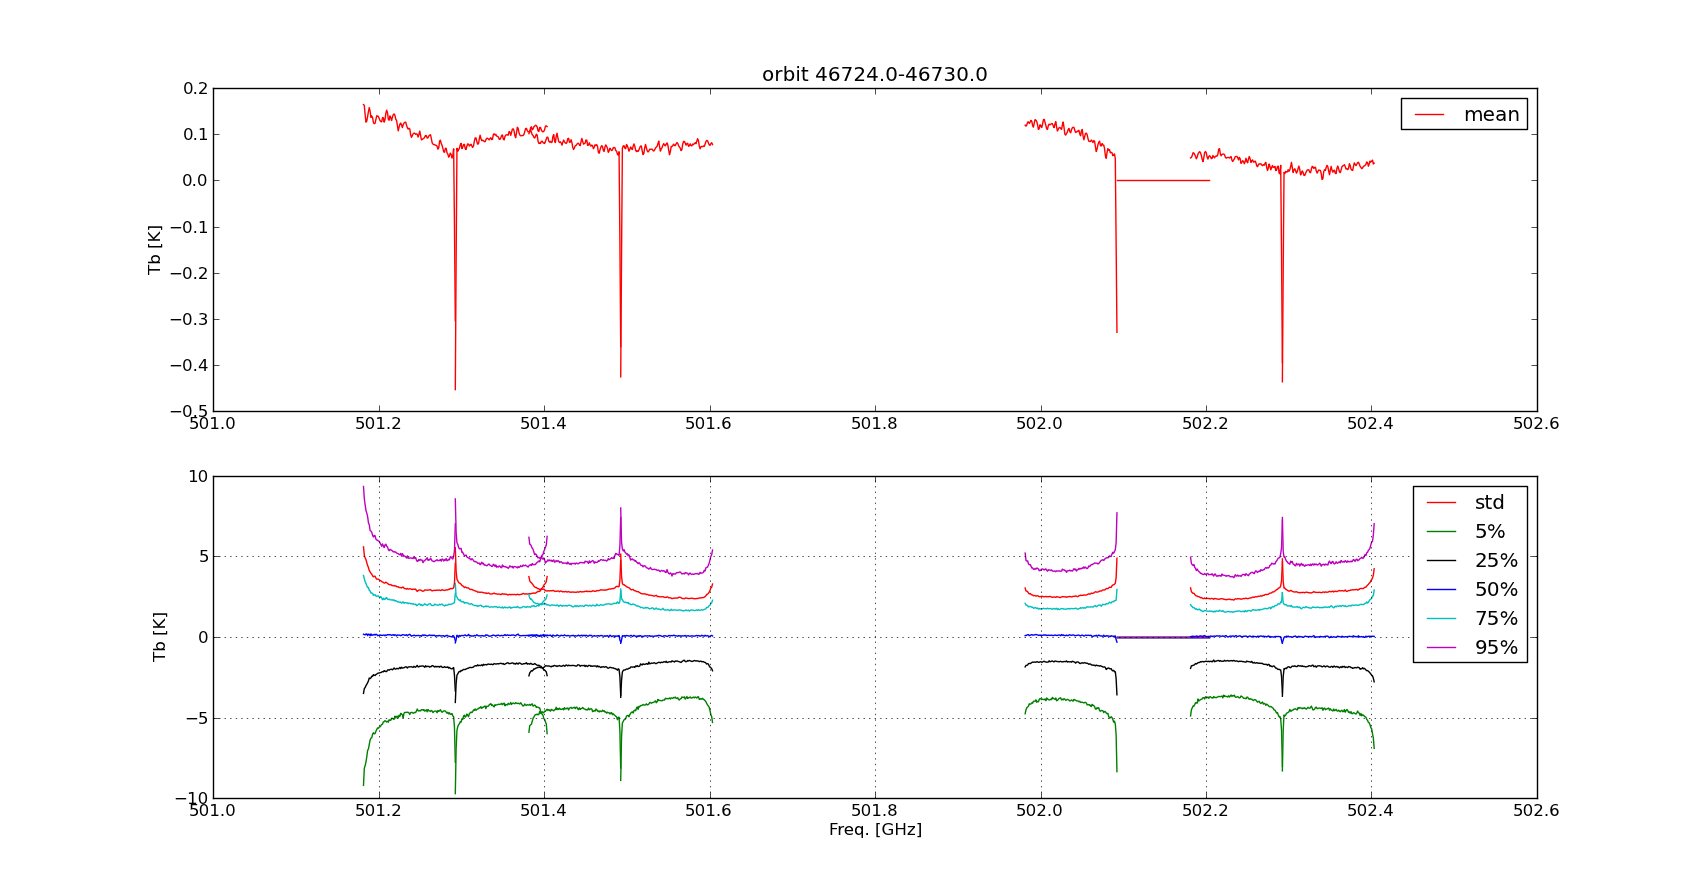
\includegraphics[scale=0.35]{study4_4.png}\\
\caption{The upper panel shows a mean spectrum of calibrated
sky signals from AC2 stratospheric mode 1,
using quadratic interpolation (x=4). 
The lower panel show a standard deviation spectrum
and percentiles spectra.}
\label{fig:study4_4.png}
\end{figure}

\begin{figure}[!t]
\centering
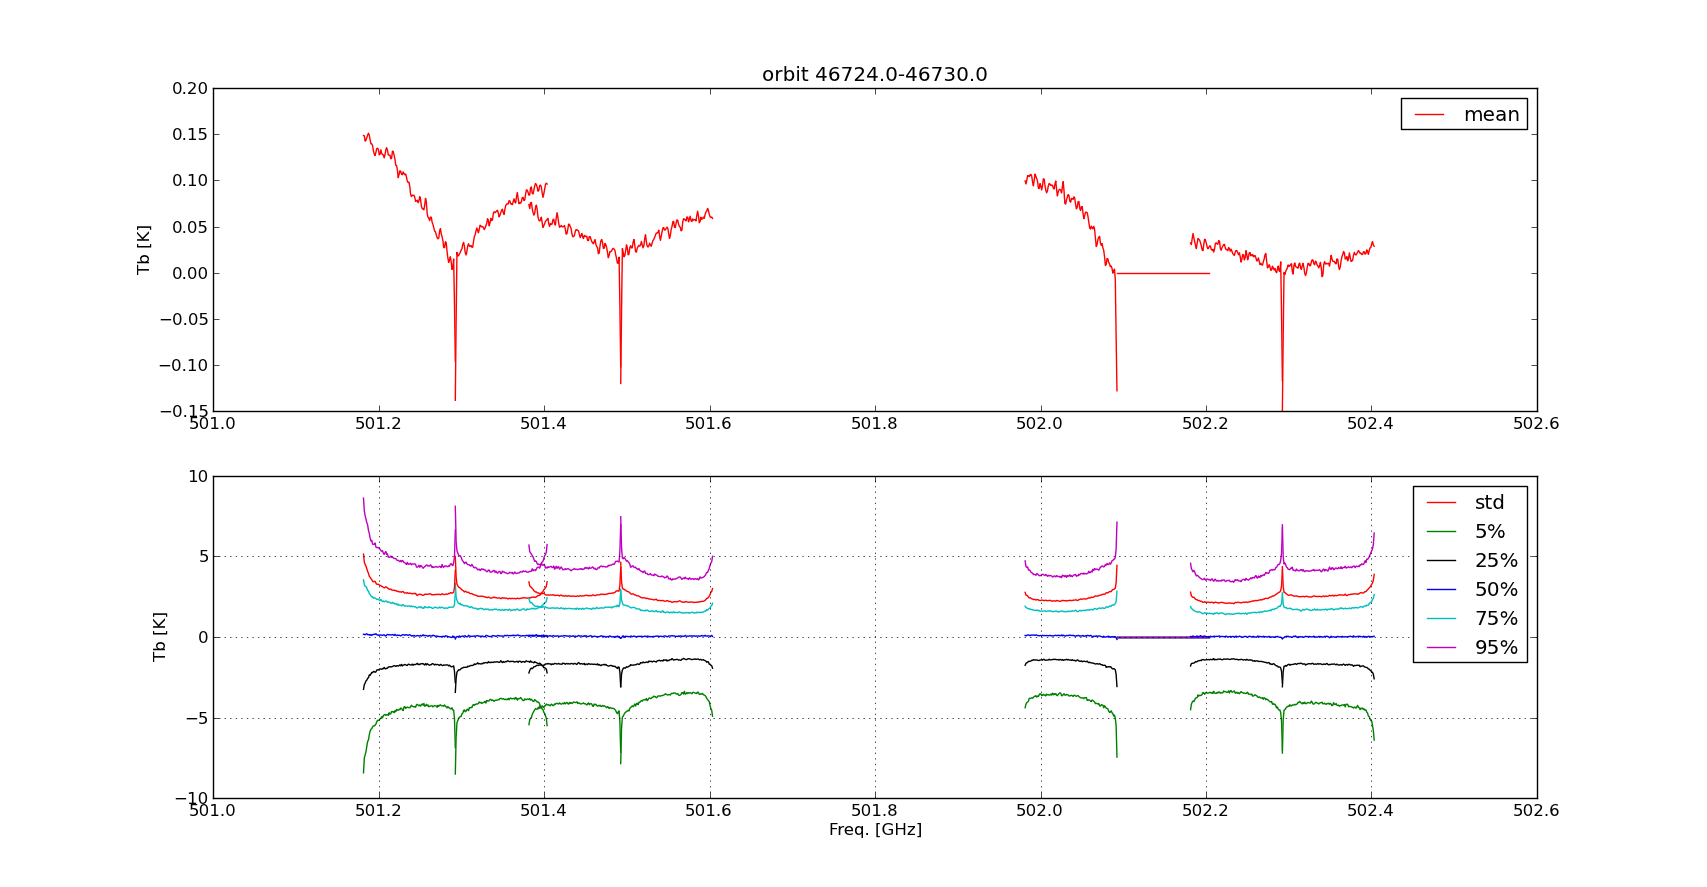
\includegraphics[scale=0.35]{study4_8.png}\\
\caption{The upper panel shows a mean spectrum of calibrated
sky signals from AC2 stratospheric mode 1,
using quadratic interpolation (x=8). 
The lower panel show a standard deviation spectrum
and percentiles spectra.}
\label{fig:study4_8.png}
\end{figure}

\begin{figure}[!t]
\centering
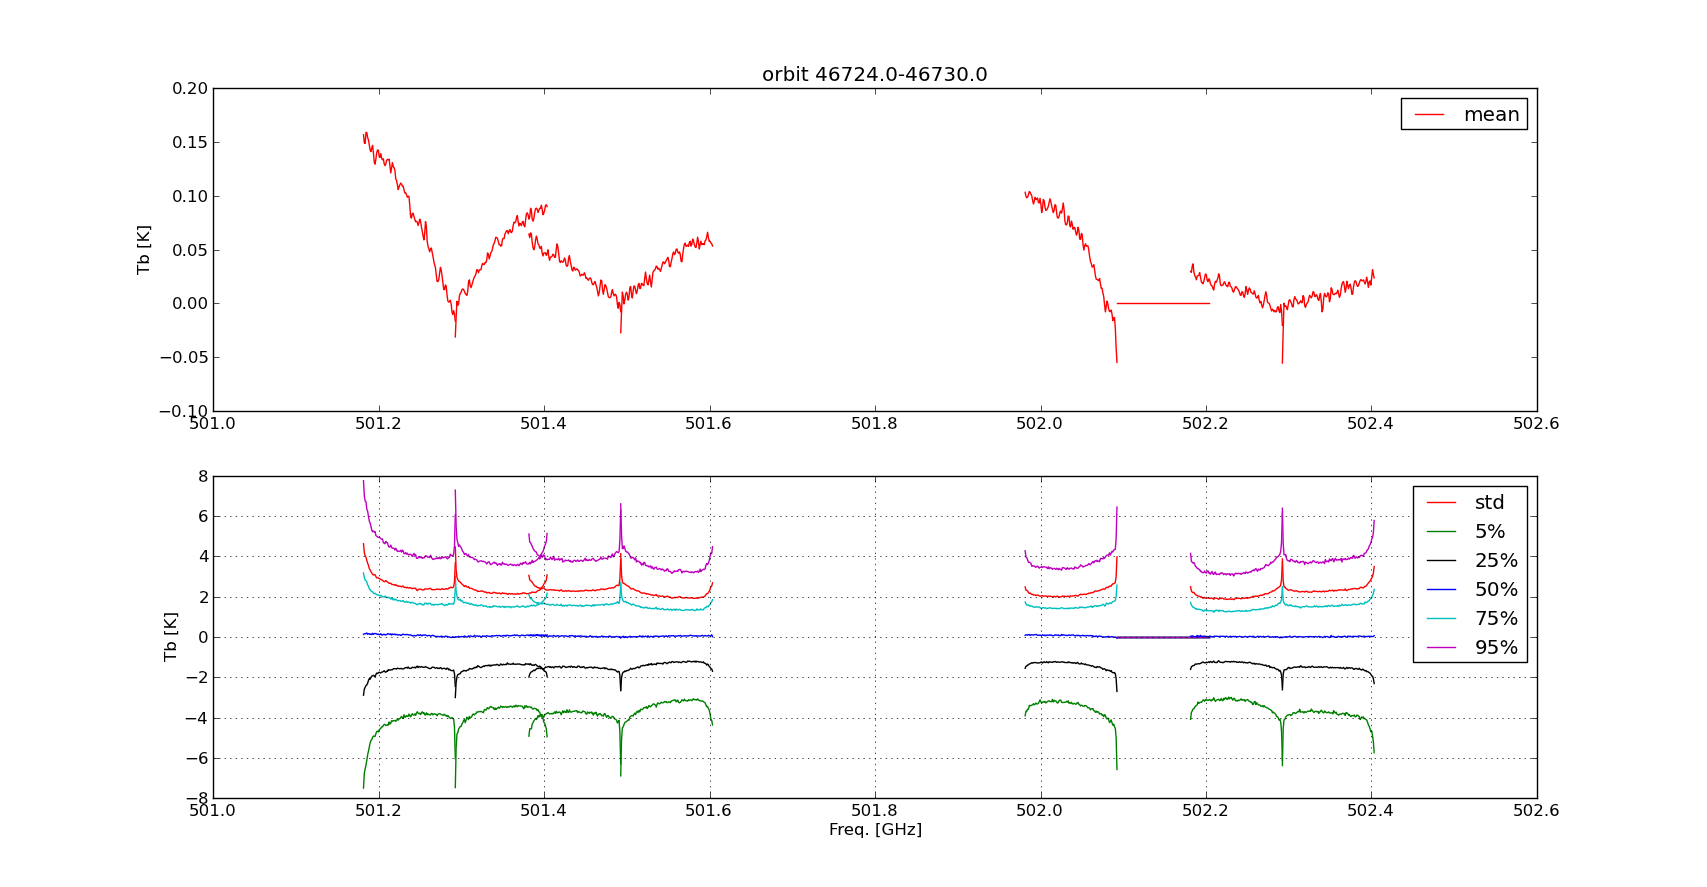
\includegraphics[scale=0.35]{study4_16.png}\\
\caption{The upper panel shows a mean spectrum of calibrated
sky signals from AC2 stratospheric mode 1,
using quadratic interpolation (x=16). 
The lower panel show a standard deviation spectrum
and percentiles spectra.}
\label{fig:study4_16.png}
\end{figure}

\begin{figure}[!t]
\centering
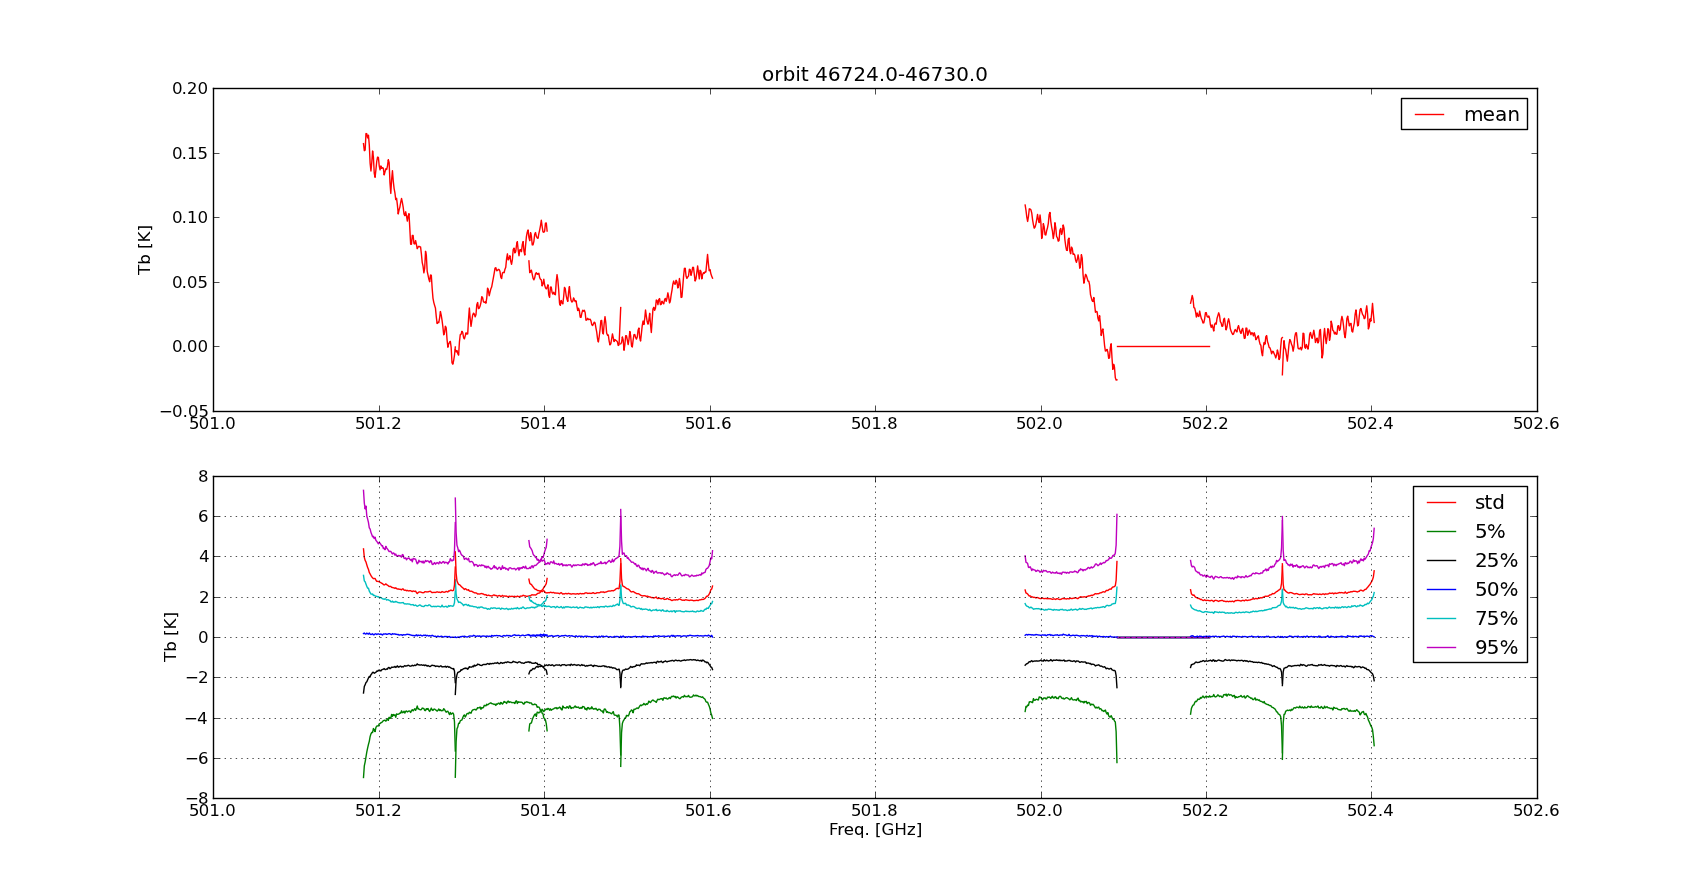
\includegraphics[scale=0.35]{study4_32.png}\\
\caption{The upper panel shows a mean spectrum of calibrated
sky signals from AC2 stratospheric mode 1,
using quadratic interpolation (x=32). 
The lower panel show a standard deviation spectrum
and percentiles spectra.}
\label{fig:study4_32.png}
\end{figure}

\begin{figure}[!t]
\centering
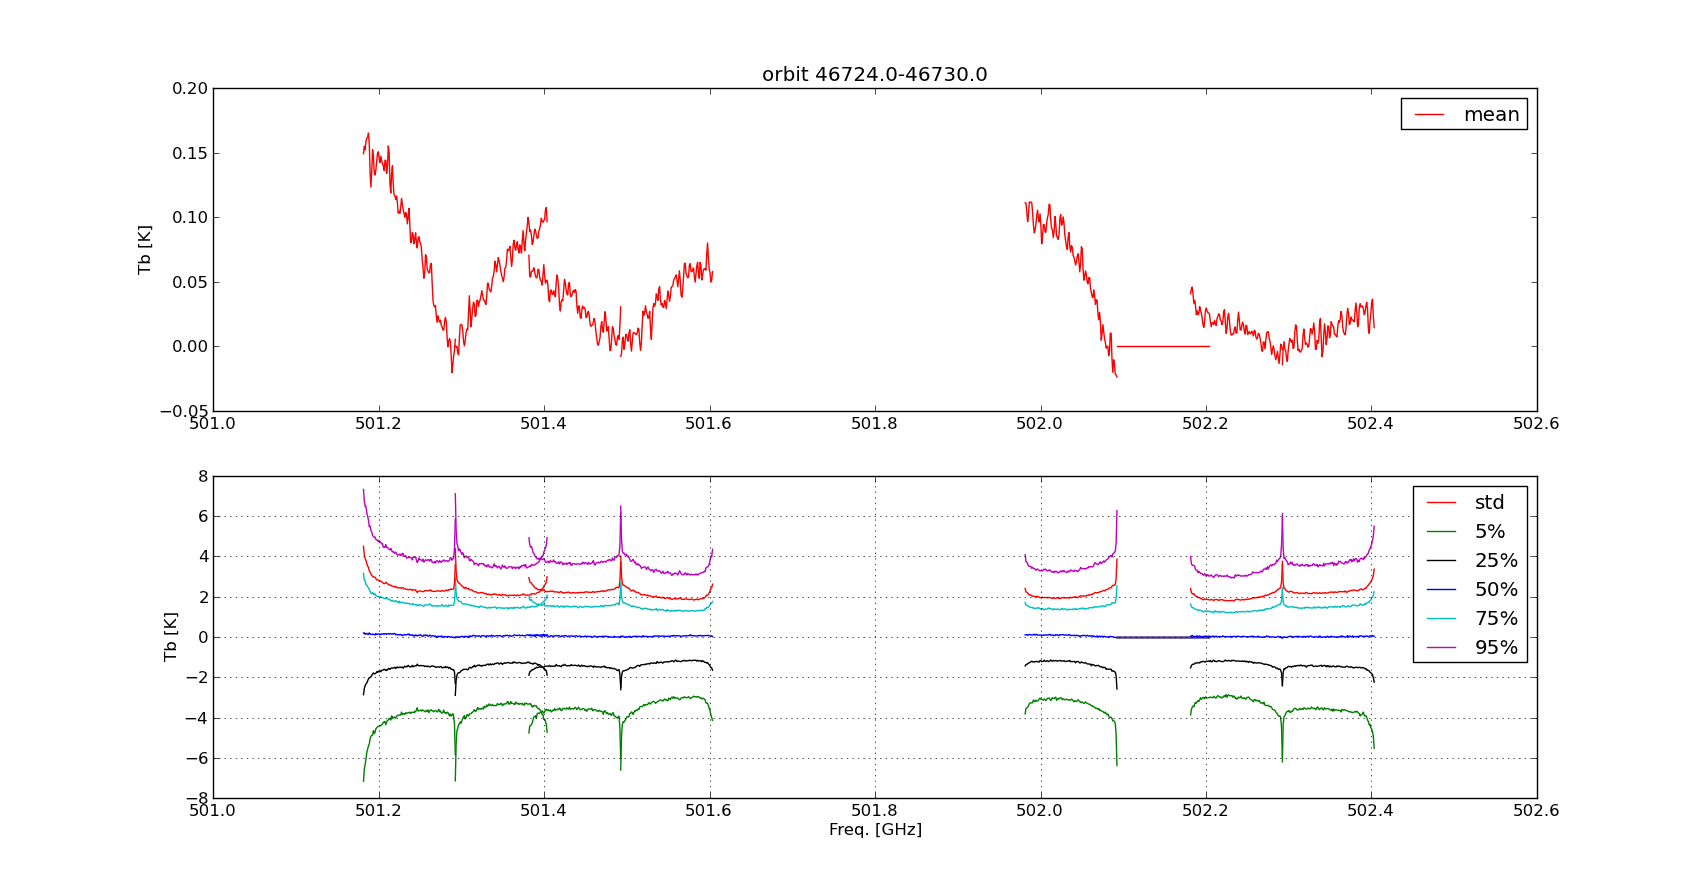
\includegraphics[scale=0.35]{study4_64.png}\\
\caption{The upper panel shows a mean spectrum of calibrated
sky signals from AC2 stratospheric mode 1,
using quadratic interpolation (x=64). 
The lower panel show a standard deviation spectrum
and percentiles spectra.}
\label{fig:study4_64.png}
\end{figure}

\begin{figure}[!t]
\centering
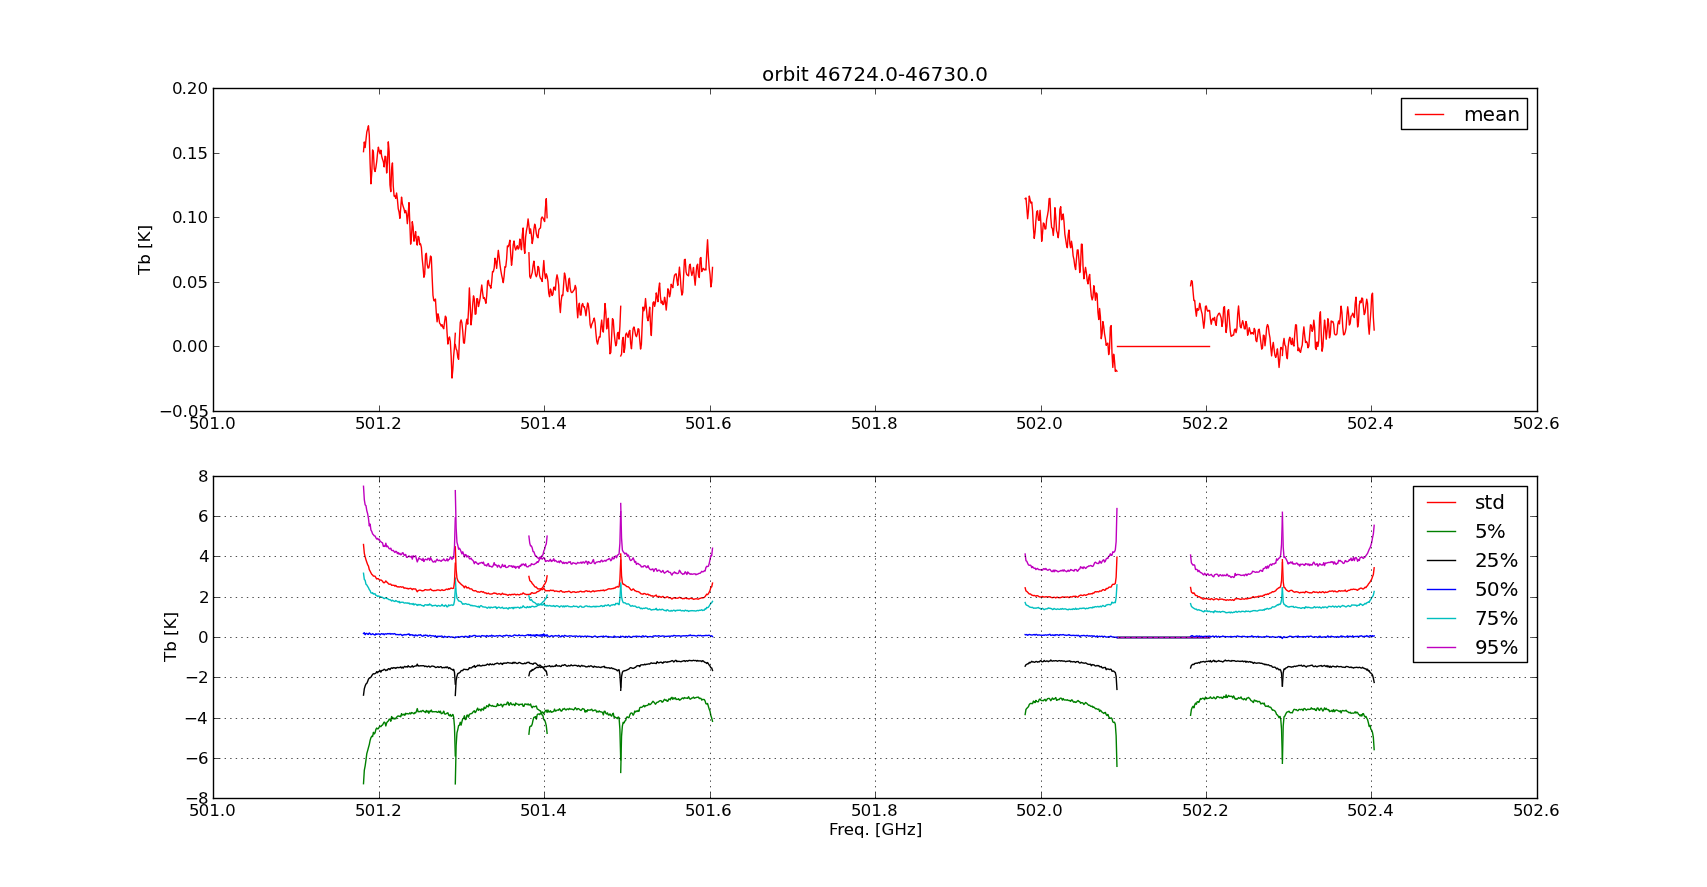
\includegraphics[scale=0.35]{study4_128.png}\\
\caption{The upper panel shows a mean spectrum of calibrated
sky signals from AC2 stratospheric mode 1,
using quadratic interpolation (x=128). 
The lower panel show a standard deviation spectrum
and percentiles spectra.}
\label{fig:study4_.png}
\end{figure}

Figures 3 to 8 show similar data as Figure 1 but using quadratic
interpolation with different setups
(weight parameter \(\lambda = \Delta T /x, x=4,8,16,32,64,128\)). 
In general, the results from the quadratic interpolations
are very similar as the result from the linear interpolation.
The same pattern in mean and median values are observed, and
similar distributions of data.
The result from x=32 setup seems to be slightly better
than for other values of x in terms of standard deviation,
and the results agree very well with the result from linear interpolation.
For such high value of \(x\) fairly few number of data
points are effectively used in the fit (see Figure 9).
Figure 9 indicates that the fit in this case should be 
very close to a linear interpolation.

   

\begin{figure}[!t]
\centering
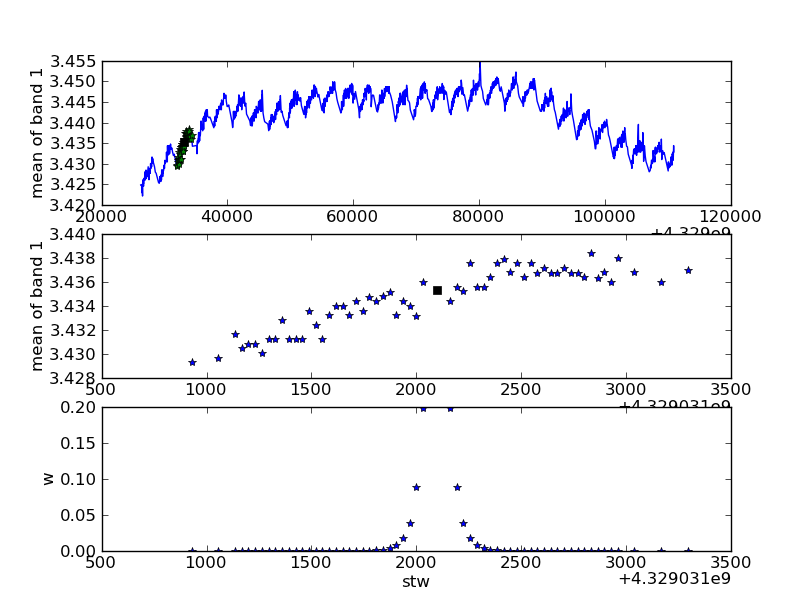
\includegraphics[scale=0.35]{study4_demo32.png}\\
\caption{The upper panel shows mean of band1 of level1a data
from several scans.
The middle panel shows a zoom in of the black dots in the upper panel,
and the black square is the fitted value
(the fit is performed for each channel). 
The lower panel shows the corresponding weights (x=32) of each measurement 
in the fit. }
\label{fig:study4_dem32.png}
\end{figure}




%\clearpage
%\newpage
\end{document}
